% \begin{document}

\chapter{Introduzione all'Intelligenza Artificiale}

\textit{Lezione 1 -- M. Milano, DISI, Università di Bologna.}
Questo capitolo copre la panoramica introduttiva del corso: che cosa si intende per
intelligenza, il test di Turing, le classificazioni dei sistemi di IA, i due grandi
approcci (simbolico e connessionista), le forme di ragionamento, la programmazione
logica, il machine learning, il planning automatico e le metafore naturali
(swarm intelligence, algoritmi genetici, reinforcement learning).

\section{Che cos'è l'intelligenza?}

\dfn{Intelligenza}{
  L'intelligenza è stata definita in molti modi, tra cui: la capacità di
  \textbf{logica}, \textbf{comprensione}, \textbf{autocoscienza},
  \textbf{apprendimento}, \textbf{conoscenza emotiva}, \textbf{ragionamento},
  \textbf{pianificazione}, \textbf{creatività}, \textbf{pensiero critico} e
  \textbf{problem solving}.

  Più in generale, può essere descritta come l'abilità di \emph{percepire o inferire
  informazione}, e di \emph{ritenerla come conoscenza} da applicare per ottenere
  \emph{comportamenti adattivi} all'interno di un ambiente o di un contesto.
}

\nt{
  La definizione è volutamente vaga: non esiste un consenso su che cosa sia
  l'intelligenza, e di conseguenza non esiste una definizione univoca di
  \emph{Intelligenza Artificiale}. Questa ambiguità è il motivo per cui Turing
  sposta la domanda dal \emph{che cos'è} al \emph{come lo riconosciamo}.
}

\section{Turing: le macchine possono pensare?}

Nel 1950 Alan Turing pubblica \emph{Computing Machinery and Intelligence}.
Il problema di partenza è duplice: definire una \textbf{macchina universale} e
definire che cosa significa \textbf{pensare} (termine ambiguo). Turing aggira il
secondo problema sostituendolo con un criterio operativo.

\dfn{Imitation game (test di Turing)}{
  Ci sono tre attori: un \textbf{umano}, un \textbf{computer} e un
  \textbf{interrogante}, collocato in una stanza diversa. L'interrogante deve
  classificare quale dei due interlocutori sia l'umano e quale la macchina,
  comunicando solo tramite testo.

  Domanda: \emph{è possibile che un computer inganni l'interrogante ed essere
  classificato come umano?}
}

Al test sono state mosse varie obiezioni; resta però il fatto che esso definisce
implicitamente una \emph{agenda di ricerca}.

\mprop{Capacità richieste dal test di Turing}{
  Per superare il test, un calcolatore deve possedere:
  \begin{enumerate}[label=(\alph*)]
    \item \textbf{Natural Language Processing} -- comprendere e produrre linguaggio;
    \item \textbf{Knowledge Representation} -- rappresentare ciò che sa;
    \item \textbf{Automatic Reasoning} -- ragionare sulla conoscenza rappresentata;
    \item \textbf{Machine Learning} -- adattarsi e generalizzare.
  \end{enumerate}
  \textbf{Oltre il test di Turing} (interazione fisica): robotica, visione
  artificiale, parlato, movimento.
}

\ex{Chatbot e test di Turing}{
  Nel 2014 il chatbot \textbf{Eugene Goostman}, che imitava le risposte di un
  ragazzino di 13 anni, ha superato il test. Altri sistemi noti: \textbf{Cleverbot}
  (Machine Intelligence Prize 2010), \textbf{SIRI} (Apple), \textbf{Cortana}
  (Microsoft), \textbf{Alexa} (Amazon), \textbf{ChatGPT} (OpenAI).

  Sono spesso costruiti indicizzando conversazioni precedenti: ciò che manca è la
  \textbf{coerenza} (da cui le \emph{allucinazioni}), lo \textbf{stato del dialogo}
  e la \textbf{semantica}.
}

\nt{
  Prospettiva metodologica: l'approccio ingegneristico privilegia
  l'\textbf{emulazione} del comportamento intelligente in domini limitati, più che
  il raggiungimento di una intelligenza \emph{reale}.
}

\subsection{Oltre il test di Turing}

Task che richiedono comprensione profonda del linguaggio, \emph{common-sense},
capacità di ragionamento e analisi multimodale:
\begin{itemize}
  \item \textbf{rompicapo matematici};
  \item \textbf{risoluzione di problemi geometrici} (Allen Institute).
\end{itemize}

\ex{Puzzle dell'Allen Institute}{
  Usando i numeri interi da 2 a 7, riempire le caselle libere in modo che la somma
  dei tre numeri attorno al cerchio nero sia 11.
}

\subsection{La previsione di Turing}

\nt{
  \textit{``I believe that in about fifty years' time it will be possible to
  programme computers, with a storage capacity of about $10^9$, to make them play
  the imitation game so well that an average interrogator will not have more than
  70\% chance of making the right identification after five minutes of questioning.
  \dots\ I believe that at the end of the century the use of words and general
  educated opinion will have altered so much that one will be able to speak of
  machines thinking without expecting to be contradicted.''}

  \hfill --- A.~Turing, \emph{Computing machinery and intelligence}, Mind, vol.~59,
  n.~236, pp.~433--460, 1950.
}

\section{Classificazione dei sistemi di IA}

\dfn{Weak AI vs Strong AI}{
  \begin{itemize}
    \item \textbf{Weak AI} -- domanda di ricerca: \emph{è possibile costruire
      sistemi che si comportano \textbf{come se} fossero intelligenti?}
    \item \textbf{Strong AI} -- domanda di ricerca: \emph{è possibile costruire
      sistemi che \textbf{sono} intelligenti?} Che abbiano menti coscienti,
      volontà e sentimenti?
  \end{itemize}
}

\dfn{General AI vs Narrow AI}{
  \begin{itemize}
    \item \textbf{General AI}: sistemi in grado di affrontare qualunque task
      generalizzato venga loro richiesto, molto come farebbe un umano.
    \item \textbf{Narrow AI}: sistemi in grado di gestire un \emph{solo} task
      particolare. Mostrano un certo grado di intelligenza in un campo specifico,
      ma restano sistemi che eseguono compiti altamente specializzati per gli umani
      all'interno di quel campo ristretto.
  \end{itemize}
}

\section{Nascita e definizioni dell'IA}

L'Intelligenza Artificiale nasce nel \textbf{1956} (Minsky, McCarthy, Shannon,
Newell, Simon).

\nt{
  \textit{``The study is to proceed on the basis of the conjecture that every aspect
  of learning or any other feature of intelligence can in principle be so precisely
  described that a machine can be made to simulate it.''} [McCarthy 1955]
}

Alcune definizioni di IA:
\begin{itemize}
  \item \textbf{Studio di come far fare ai computer le cose che gli umani fanno
    meglio.} È una definizione \emph{transitoria}: si pensi agli scacchi, dove
    l'uomo non è più il migliore.
  \item \textbf{Studio di come costruire computer che superino il test di Turing}
    (ragionamento, comprensione del linguaggio naturale, apprendimento). Se il
    sistema è situato in un ambiente si aggiungono percezione, visione, movimento,
    robotica.
  \item Altre definizioni non si legano direttamente all'intelligenza umana, ma
    all'\textbf{abilità di interagire con un ambiente e di adattarvisi}.
\end{itemize}

\section{Breve storia dell'IA}

\begin{itemize}
  \item \textbf{1943--1956 -- La nascita dell'IA.} Reti neurali, programmi per gli
    scacchi, dimostratori di teoremi.
  \item \textbf{1952--1969 -- Entusiasmo iniziale e grandi aspettative.}
    General Problem Solver, linguaggio LISP, reti neurali.
  \item \textbf{1966--1974 -- Ritorno con i piedi per terra.} Alcuni programmi non
    erano adeguati (ELIZA, traduzioni sintattiche, reti neurali), altri erano troppo
    costosi computazionalmente (\textbf{esplosione combinatoria}).
  \item \textbf{1969--1979 -- Sistemi basati su conoscenza.} Conoscenza profonda in
    un dominio limitato: \textbf{sistemi esperti}.
  \item \textbf{1980--1988 -- L'IA entra nell'industria.} Sistemi esperti
    commercialmente di successo, progetto giapponese di \emph{quinta generazione},
    aziende che lavorano sull'IA, fondi di ricerca.
  \item \textbf{1988--2010 -- Era del Web e di Internet.} Sistemi di supporto alle
    decisioni, agenti robotici, linguaggio naturale.
  \item \textbf{2010--oggi -- Machine learning e deep learning.} Big data e potenza
    di calcolo massiva hanno reso funzionanti le reti profonde. Intelligenza e
    percezione aumentate, interesse industriale, industria 4.0.
  \item \textbf{2020--oggi -- IA generativa e agenti conversazionali.}
\end{itemize}

\section{I due approcci principali all'IA}

\dfn{Approccio top-down (simbolico)}{
  \begin{itemize}
    \item Rappresentazione \textbf{simbolica} della conoscenza;
    \item logiche, ontologie, sistemi a regole, architettura \textbf{dichiarativa};
    \item modelli \textbf{comprensibili all'uomo}.
  \end{itemize}
}

\dfn{Approccio bottom-up (connessionista)}{
  \begin{itemize}
    \item \textbf{Reti neurali}. La conoscenza non è simbolica ed è ``codificata''
      nelle connessioni tra i neuroni;
    \item i concetti sono \textbf{appresi da esempi};
    \item i modelli \textbf{non sono comprensibili} all'uomo.
  \end{itemize}
}

\section{Ragionamento e logica}

\dfn{Ragionamento deduttivo}{
  Sillogismo aristotelico, logica deduttiva.
  Da \emph{Tutti gli uomini sono mortali} e \emph{Socrate è un uomo} segue
  \emph{Socrate è mortale}.

  È \textbf{corretto}, ma non permette di ``imparare'' nuova conoscenza.
}

\dfn{Ragionamento induttivo}{
  Apprendimento, \emph{deduzione inversa}.
  Dall'osservazione che diversi uccelli volano si conclude che \emph{tutti gli
  uccelli volano} (e i pinguini?).

  Produce \textbf{nuova conoscenza} a scapito della \textbf{correttezza}.
}

\dfn{Ragionamento ipotetico o abduttivo}{
  Duale del deduttivo. Dall'osservazione della \emph{morte di Socrate} e sapendo che
  \emph{tutti gli uomini sono mortali}, si ipotizza che \emph{Socrate sia un uomo}
  (e se fosse un gatto?).

  Risale alle \textbf{cause} attraverso l'osservazione degli \textbf{effetti}, a
  scapito della correttezza.
}

\dfn{Ragionamento per analogia}{
  Metaforico, \emph{case-based}. Non richiede un modello né molti dati, ma usa il
  \textbf{principio di similarità}: Socrate e John ``si assomigliano''; se Socrate
  ama la filosofia allora anche John ama la filosofia.

  Algoritmi tipici: \textbf{K-Nearest-Neighbor} e \textbf{Support Vector Machine}.
}

\dfn{Constraint reasoning e ottimizzazione}{
  Ragionamento basato su \textbf{vincoli}, \textbf{probabilità} e \textbf{statistica}
  (teorema di Bayes).
}

\section{Logica, dimostrazione automatica e Prolog}

Lo schema concettuale che lega logica e dimostrazione automatica è il seguente:
la \textbf{sintassi} manipola simboli \emph{non interpretati}; la \textbf{semantica}
fornisce un'\emph{interpretazione}; i due mondi sono collegati dalle proprietà di
\textbf{correttezza} (\emph{soundness}) e \textbf{completezza}.

\begin{figure}[H]
  \centering
  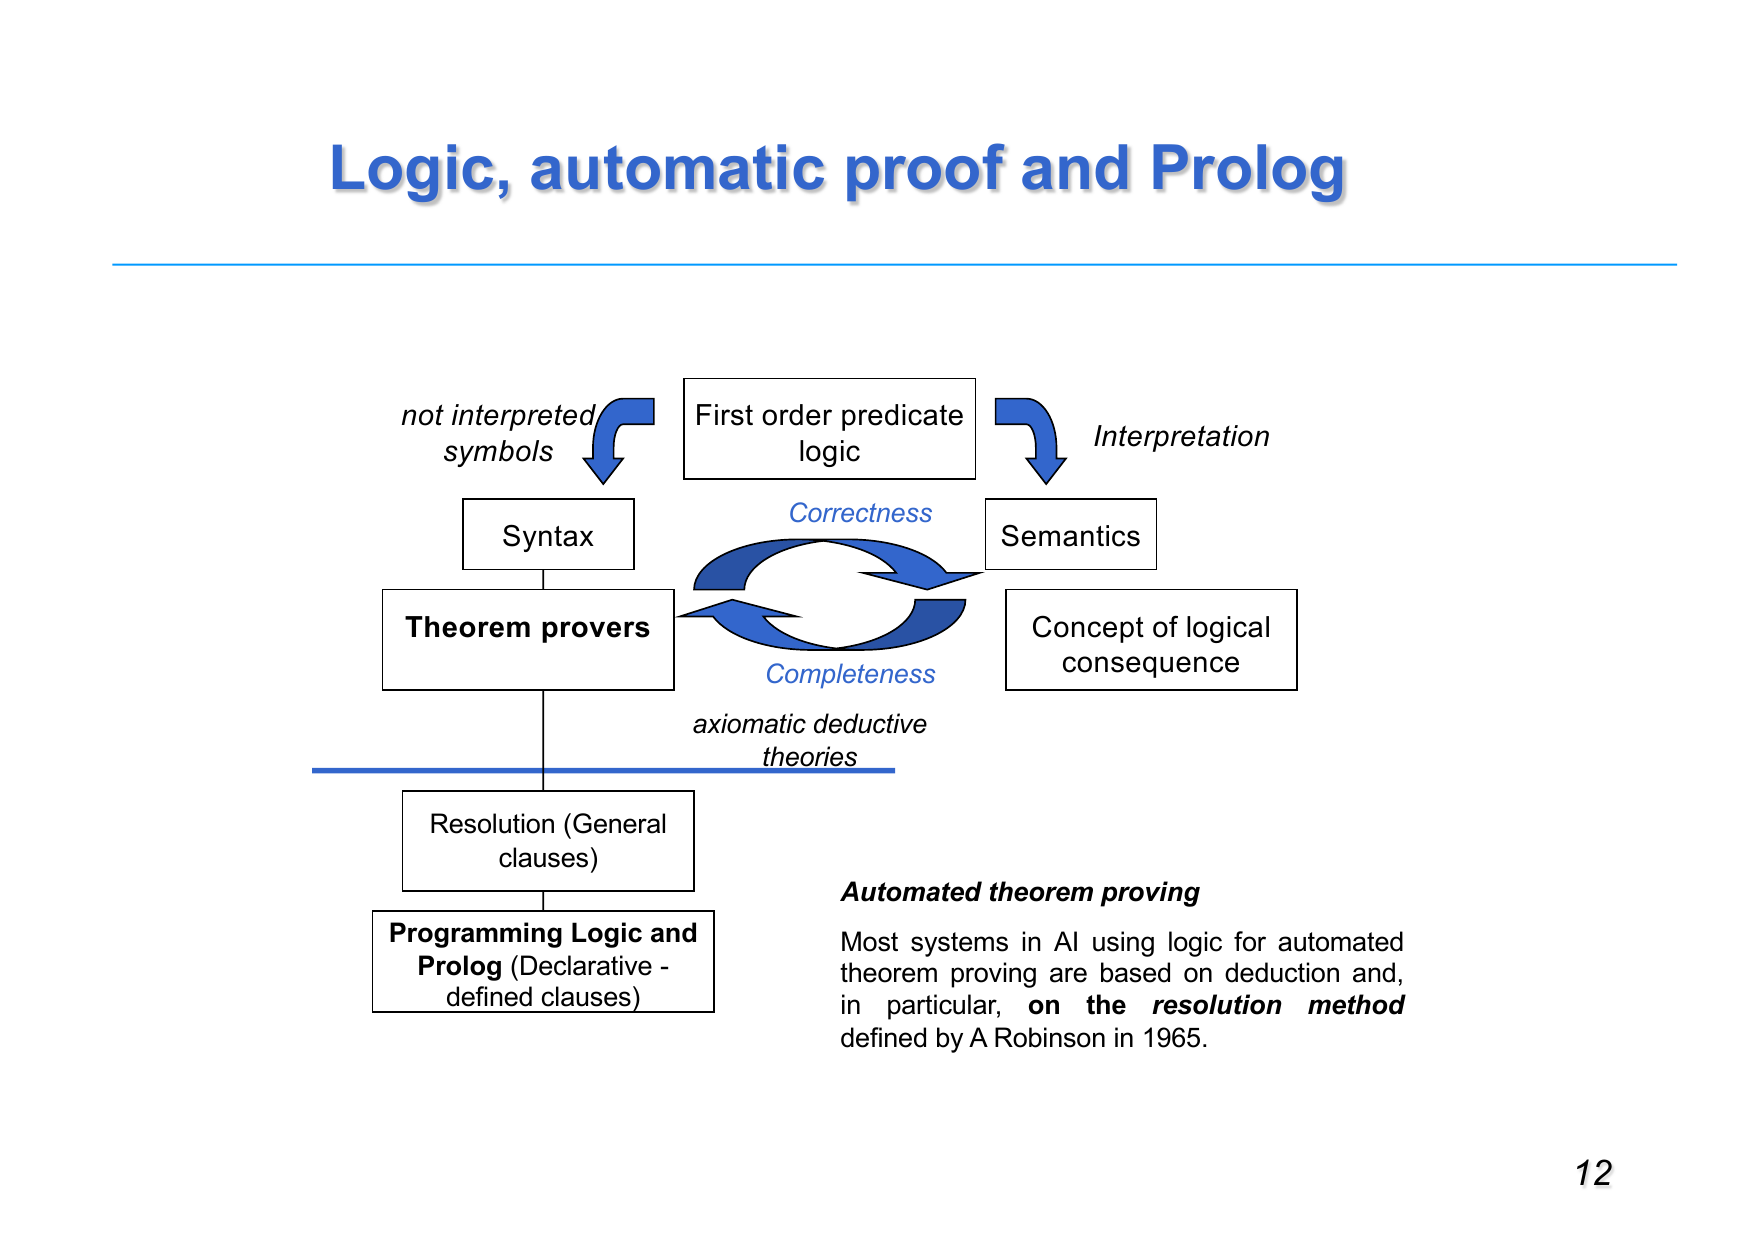
\includegraphics[width=0.85\textwidth]{img/logica-prolog.png}
  \caption{Dalla logica del primo ordine ai theorem prover e a Prolog.}
\end{figure}

\thm{Risoluzione}{
  La maggior parte dei sistemi di IA che usano la logica per la dimostrazione
  automatica di teoremi si basa sulla \textbf{deduzione} e, in particolare, sul
  \textbf{metodo di risoluzione} definito da A.~Robinson nel \textbf{1965}.
}

\nt{
  La catena è: logica del primo ordine $\to$ teorie assiomatiche deduttive $\to$
  risoluzione su \textbf{clausole generali} $\to$ programmazione logica e Prolog,
  che si restringe alle \textbf{clausole definite} (Horn) per ottenere efficienza.
}

\subsection{Tre letture del concetto di algoritmo}

\dfn{Interpretazioni di ``algoritmo''}{
  \begin{enumerate}
    \item Algoritmo = \textbf{strutture dati + istruzioni};
    \item Algoritmo = \textbf{logica (conoscenza) + controllo (motore inferenziale)};
    \item Algoritmo = \textbf{esempi (esperienza) + machine learning}.
  \end{enumerate}
  Scendendo nella lista aumentano il \textbf{livello di generalità} e
  l'``\textbf{intelligenza}''.
}

\subsection{Linguaggi dichiarativi e Prolog}

\dfn{Algoritmo = Logica + Controllo}{
  La conoscenza sul problema è \textbf{indipendente dal suo uso}:
  \begin{itemize}
    \item esprime il \textbf{COSA} e non il \textbf{COME};
    \item alta \textbf{modularità} e \textbf{flessibilità};
    \item è lo schema di progetto alla base della maggior parte dei
      \textbf{sistemi basati su conoscenza} (sistemi esperti).
  \end{itemize}
  \textbf{LOGICA}: la conoscenza sul problema determina \emph{correttezza} ed
  \emph{efficienza}.\\
  \textbf{CONTROLLO}: la strategia di soluzione determina l'\emph{efficienza}.
}

\nt{
  \textbf{PROLOG} = \emph{PROgramming in LOGic}. È il più noto linguaggio di
  programmazione logica; nasce dalle idee di \textbf{R.~Kowalski} e dalla prima
  realizzazione di \textbf{A.~Colmerauer} (1973).
}

\subsection{Struttura di un programma Prolog}

\dfn{Programma Prolog}{
  Un programma Prolog è un insieme di \textbf{clausole di Horn} che rappresentano:
  \begin{itemize}
    \item \textbf{FATTI} sugli oggetti in esame e sulle relazioni;
    \item \textbf{REGOLE} su oggetti e relazioni (IF \dots\ THEN);
    \item \textbf{GOAL} (clausole senza testa), sulla base della conoscenza definita.
  \end{itemize}
  Una regola ha la forma \texttt{Testa :- Corpo}.
}

\begin{Example}{Colleghi di lavoro}{}
  Due individui sono colleghi se lavorano per la stessa azienda.
\begin{lstlisting}
colleague(X,Y) :- works(X,Z), works(Y,Z), different(X,Y).   % REGOLA

works(emp1,ibm).
works(emp2,ibm).
works(emp3,txt).            % FATTI
works(emp4,olivetti).
works(emp5,txt).

:- colleague(X,Y).          % GOAL
\end{lstlisting}
\end{Example}

\begin{Example}{Somma di due interi (definizione dichiarativa)}{}
\begin{lstlisting}
sum(0,X,X).                         % FATTO
sum(s(X),Y,s(Z)) :- sum(X,Y,Z).     % REGOLA
\end{lstlisting}
  \begin{itemize}
    \item \texttt{sum} è un simbolo \textbf{non interpretato};
    \item i numeri interi sono definiti con la struttura \textbf{successore}
      \texttt{s(X)};
    \item la definizione è \textbf{ricorsiva}.
  \end{itemize}
  Lo stesso programma ammette \textbf{molte query diverse}, cioè molti algoritmi:
\begin{lstlisting}
:- sum(s(0),s(s(0)),Y).                  % somma
:- sum(s(0),Y,s(s(s(0)))).               % sottrazione
:- sum(X,Y,s(s(s(0)))).                  % tutte le decomposizioni di 3
:- sum(X,Y,Z).                           % tutte le triple
:- sum(X,Y,s(s(s(0)))), sum(X,s(0),Y).   % sistema di vincoli
\end{lstlisting}
\end{Example}

\nt{
  Questo è il punto chiave della dichiaratività: \textbf{un solo programma, molti
  algoritmi}. Cambiando quali argomenti sono in input e quali in output si ottengono
  comportamenti diversi senza riscrivere il codice.
}

\subsection{Deduzione e induzione in programmazione logica}

Si usano tre insiemi: la \textbf{teoria} $T$ (le regole), la \textbf{background
knowledge} $B$ (i fatti noti) e gli \textbf{esempi} $E$.

\dfn{Deduzione}{
  Dati $T$ e $B$, si deriva $E$: $\quad T \cup B \models E$.
  \begin{center}
  \begin{tabular}{p{0.3\textwidth}|p{0.28\textwidth}|p{0.3\textwidth}}
    \textbf{$T$ (teoria)} & \textbf{$B$ (background)} & \textbf{$E$ (dedotto)}\\
    \hline
    \texttt{parent(X,Y):-mother(X,Y).} & \texttt{mother(mary,vinni).}
      & \texttt{parent(mary,vinni).}\\
    \texttt{parent(X,Y):-father(X,Y).} & \texttt{mother(mary,andre).}
      & \texttt{parent(mary,andre).}\\
      & \texttt{father(carrey,vinni).} & \texttt{parent(carrey,vinni).}\\
      & \texttt{father(carrey,andre).} & \texttt{parent(carrey,andre).}\\
  \end{tabular}
  \end{center}
}

\dfn{Induzione}{
  Dati $B$ e gli esempi \textbf{positivi} $E^+$ (e \textbf{negativi} $E^-$), si
  induce la teoria $T$:
  \begin{center}
  \begin{tabular}{p{0.3\textwidth}|p{0.28\textwidth}|p{0.3\textwidth}}
    \textbf{$E^+$ / $E^-$} & \textbf{$B$ (background)} & \textbf{$T$ (indotta)}\\
    \hline
    \texttt{parent(mary,vinni).} & \texttt{mother(mary,vinni).}
      & \texttt{parent(X,Y):-mother(X,Y).}\\
    \texttt{parent(mary,andre).} & \texttt{mother(mary,andre).}
      & \texttt{parent(X,Y):-father(X,Y).}\\
    \texttt{parent(carrey,vinni).} & \texttt{father(carrey,vinni).} & \\
    \texttt{parent(carrey,andre).} & \texttt{father(carrey,andre).} & \\
    \hline
    \texttt{parent(mary,carrey).} $\in E^-$ & & \\
  \end{tabular}
  \end{center}
  Le condizioni che $T$ deve soddisfare sono:
  \[
    \forall e^+ \in E^+ : \; B \cup T \models e^+
    \qquad (T \text{ è \textbf{completa}})
  \]
  \[
    \forall e^- \in E^- : \; B \cup T \not\models e^-
    \qquad (T \text{ è \textbf{consistente}})
  \]
}

\nt{
  L'induzione è dunque \textbf{deduzione inversa}: si cerca la teoria che, insieme
  alla background knowledge, \emph{spiega} tutti gli esempi positivi e
  \emph{nessuno} di quelli negativi. Questo è il cuore dell'\textbf{Inductive Logic
  Programming}.
}

\subsection{Abduzione in programmazione logica}

\begin{Definition}[colbacktitle=red!75!black]{Abduzione}{}
  Dati la teoria $T$ e le osservazioni $E$, si cercano le \textbf{ipotesi} $B$ tali
  che $T \cup B \models E$.

  Con $T = \{\texttt{parent(X,Y):-mother(X,Y).},\ \texttt{parent(X,Y):-father(X,Y).}\}$
  e $E = \{\texttt{parent(mary,vinni)}, \dots\}$ si ottengono ipotesi
  \textbf{disgiuntive}:
\begin{lstlisting}
mother(mary,vinni) v father(mary,vinni).
mother(mary,andre) v father(mary,andre).
mother(carrey,vinni) v father(carrey,vinni).
mother(carrey,andre) v father(carrey,andre).
\end{lstlisting}
\end{Definition}

Per \textbf{controllare le ipotesi} si usano spesso i \textbf{vincoli di integrità}
(\emph{integrity constraints}, IC).

\begin{Example}{Abduzione con vincoli di integrità}{}
  Aggiungendo alla teoria i vincoli
\begin{lstlisting}
mother(X,Y) -> female(X).
father(X,Y) -> male(X).
female(mary).
male(carrey).
\end{lstlisting}
  le ipotesi disgiuntive collassano in ipotesi \textbf{determinate}:
\begin{lstlisting}
mother(mary,vinni).
mother(mary,andre).
father(carrey,vinni).
father(carrey,andre).
\end{lstlisting}
  Le condizioni sono ora: $\; T \cup B \models E \;$ e $\; T \cup B \models IC$.
\end{Example}

\subsection{Prolog: successi e limiti}

\begin{itemize}
  \item Grande idea rivoluzionaria: il linguaggio \textbf{non è legato
    all'architettura di Von Neumann};
  \item contrapposizione \textbf{europea} vs \textbf{americana};
  \item progetto giapponese di \textbf{quinta generazione} negli anni '80
    (fallito);
  \item nel frattempo la tecnologia ha fatto passi da gigante\dots
  \item \emph{perché Prolog non si è diffuso come si credeva negli anni '80?}
  \item molte applicazioni, idee, ricerca ed estensioni di Prolog nell'IA, ma non
    tutto.
\end{itemize}

\nt{
  Implementazioni notevoli:
  \begin{itemize}
    \item \textbf{SWI Prolog} -- molto usato e ben integrato con il Semantic Web
      (\url{http://www.swi-prolog.org});
    \item \textbf{tuProlog} -- Prolog basato su Java per applicazioni Internet,
      sviluppato a Unibo (\url{http://apice.unibo.it/xwiki/bin/view/Tuprolog/}).
  \end{itemize}
}

\section{Machine learning}

Imparare dall'esperienza, dai propri errori, dai maestri, per imitazione, è una
caratteristica peculiare dell'intelligenza. È un approccio \textbf{empirista}, che si
oppone all'approccio \textbf{razionalista}.

\dfn{Apprendimento (Michalski, 1986)}{
  \textit{Learning is constructing or modifying representations of what is being
  experienced.}
}

\dfn{Apprendimento (Simon, 1984)}{
  \textit{Learning denotes changes in the system that are adaptive in the sense that
  they enable the system to do the same task or tasks drawn from the same population
  more efficiently and more effectively the next time.}
}

\nt{
  Il machine learning è uno dei temi caldi dell'IA: tutte le maggiori aziende ICT
  investono e assumono persone con background in ML (Google, Facebook, IBM, Baidu,
  Disney, \dots). \textbf{Perché?} Perché hanno \textbf{molti dati} e vogliono
  \textbf{estrarne valore}: è l'era dei \emph{big data}.
}

\subsection{Le tre grandi famiglie}

\dfn{Supervised Learning}{
  Parte da un insieme di esempi forniti da un ``maestro'' (il \textbf{training set}).
  Risolve problemi di \textbf{classificazione} e \textbf{regressione}
  (es.\ riconoscimento di pattern).
}

\dfn{Unsupervised Learning}{
  Procede per \textbf{osservazione e scoperta}. Dall'esterno non riceve alcun aiuto:
  è il sistema stesso a dover analizzare l'informazione disponibile, classificarla e
  strutturarla, scoprendo \textbf{pattern}. Task tipici: \textbf{clustering} e
  \textbf{data mining}.
}

\dfn{Reinforcement Learning}{
  Apprende il \textbf{comportamento ottimo} dalle esperienze passate. Osserva le
  scelte buone e cattive fatte (attraverso \textbf{ricompense} e \textbf{punizioni})
  e modifica il comportamento di conseguenza. Impara principalmente
  \textbf{dagli errori}; trova molte applicazioni in robotica.
}

\subsection{Che cosa si può fare con il machine learning?}

\begin{itemize}
  \item classificare le e-mail in arrivo come \textbf{spam} o non spam;
  \item predire il \textbf{prezzo delle azioni} Apple;
  \item formulare una \textbf{diagnosi} a partire dagli esami di un paziente;
  \item riconoscere \textbf{numeri di partita IVA} scritti a mano
    [LeCun et al., 1989];
  \item insegnare a un \textbf{robot} ad afferrare una tazza;
  \item progettare una \textbf{molecola} con proprietà specifiche;
  \item \textbf{tradurre} un testo;
  \item \textbf{convertire la voce} in testo;
  \item generare automaticamente la \textbf{didascalia} di una figura;
  \item \textbf{battere il campione del mondo} in un gioco.
\end{itemize}

\subsection{Task: classificazione}

\dfn{Classificazione}{
  La classificazione è il task di approssimare una funzione di mapping $f$ da
  variabili di input $X$ a variabili di output \textbf{discrete/categoriche} $y$.

  Le variabili di output sono spesso chiamate \textbf{label}, \textbf{categorie} o
  \textbf{classi}. La funzione di mapping predice la classe o categoria di una data
  osservazione. È un task di apprendimento \textbf{supervisionato}.
}

\mprop{Varianti del problema di classificazione}{
  \begin{itemize}
    \item un problema di classificazione richiede che gli esempi siano classificati
      in una tra due o più classi;
    \item le variabili di input possono essere \textbf{reali} o \textbf{discrete};
    \item con due classi si parla di \textbf{two-class} o \textbf{binary
      classification}; con più di due classi di \textbf{multi-class};
    \item se a un esempio sono assegnate \emph{più} classi si parla di
      \textbf{multi-label classification};
    \item la \textbf{classification accuracy} è la percentuale di esempi
      correttamente classificati sul totale delle predizioni.
  \end{itemize}
}

\subsection{Task: regressione}

\dfn{Regressione}{
  La regressione è il task di approssimare una funzione di mapping $f$ da variabili
  di input $X$ a una variabile di output \textbf{continua} $y$.

  Una variabile di output continua è un valore reale (intero o floating point):
  tipicamente quantità, come importi e dimensioni. È un task
  \textbf{supervisionato}.
}

\mprop{Varianti del problema di regressione}{
  \begin{itemize}
    \item un problema di regressione richiede la predizione di una \textbf{quantità};
    \item le variabili di input possono essere reali o discrete;
    \item con più variabili di input si parla di \textbf{multivariate regression};
    \item se le variabili di input sono \textbf{ordinate nel tempo} si parla di
      \textbf{time series forecasting};
    \item poiché il modello predice una quantità, la bontà del modello va riportata
      come \textbf{errore} sulle predizioni, ad esempio l'\textbf{RMSE}.
  \end{itemize}
}

\subsection{Task: clustering}

\dfn{Clustering}{
  Il clustering è il problema di organizzare oggetti in \textbf{gruppi} i cui membri
  sono simili in qualche modo. Determina il \textbf{raggruppamento intrinseco} in un
  insieme di dati \textbf{non etichettati}: è il principale task di apprendimento
  \textbf{non supervisionato}.
}

\dfn{Tipi di clustering}{
  \begin{itemize}
    \item \textbf{Hard clustering}: ogni elemento può essere assegnato a uno e un
      solo gruppo;
    \item \textbf{Soft} o \textbf{fuzzy clustering}: ogni elemento può appartenere a
      più gruppi.
  \end{itemize}
  L'algoritmo più usato per l'hard clustering è \textbf{k-means}
  (MacQueen, 1967).
}

\section{Apprendimento simbolico e sub-simbolico}

\begin{figure}[H]
  \centering
  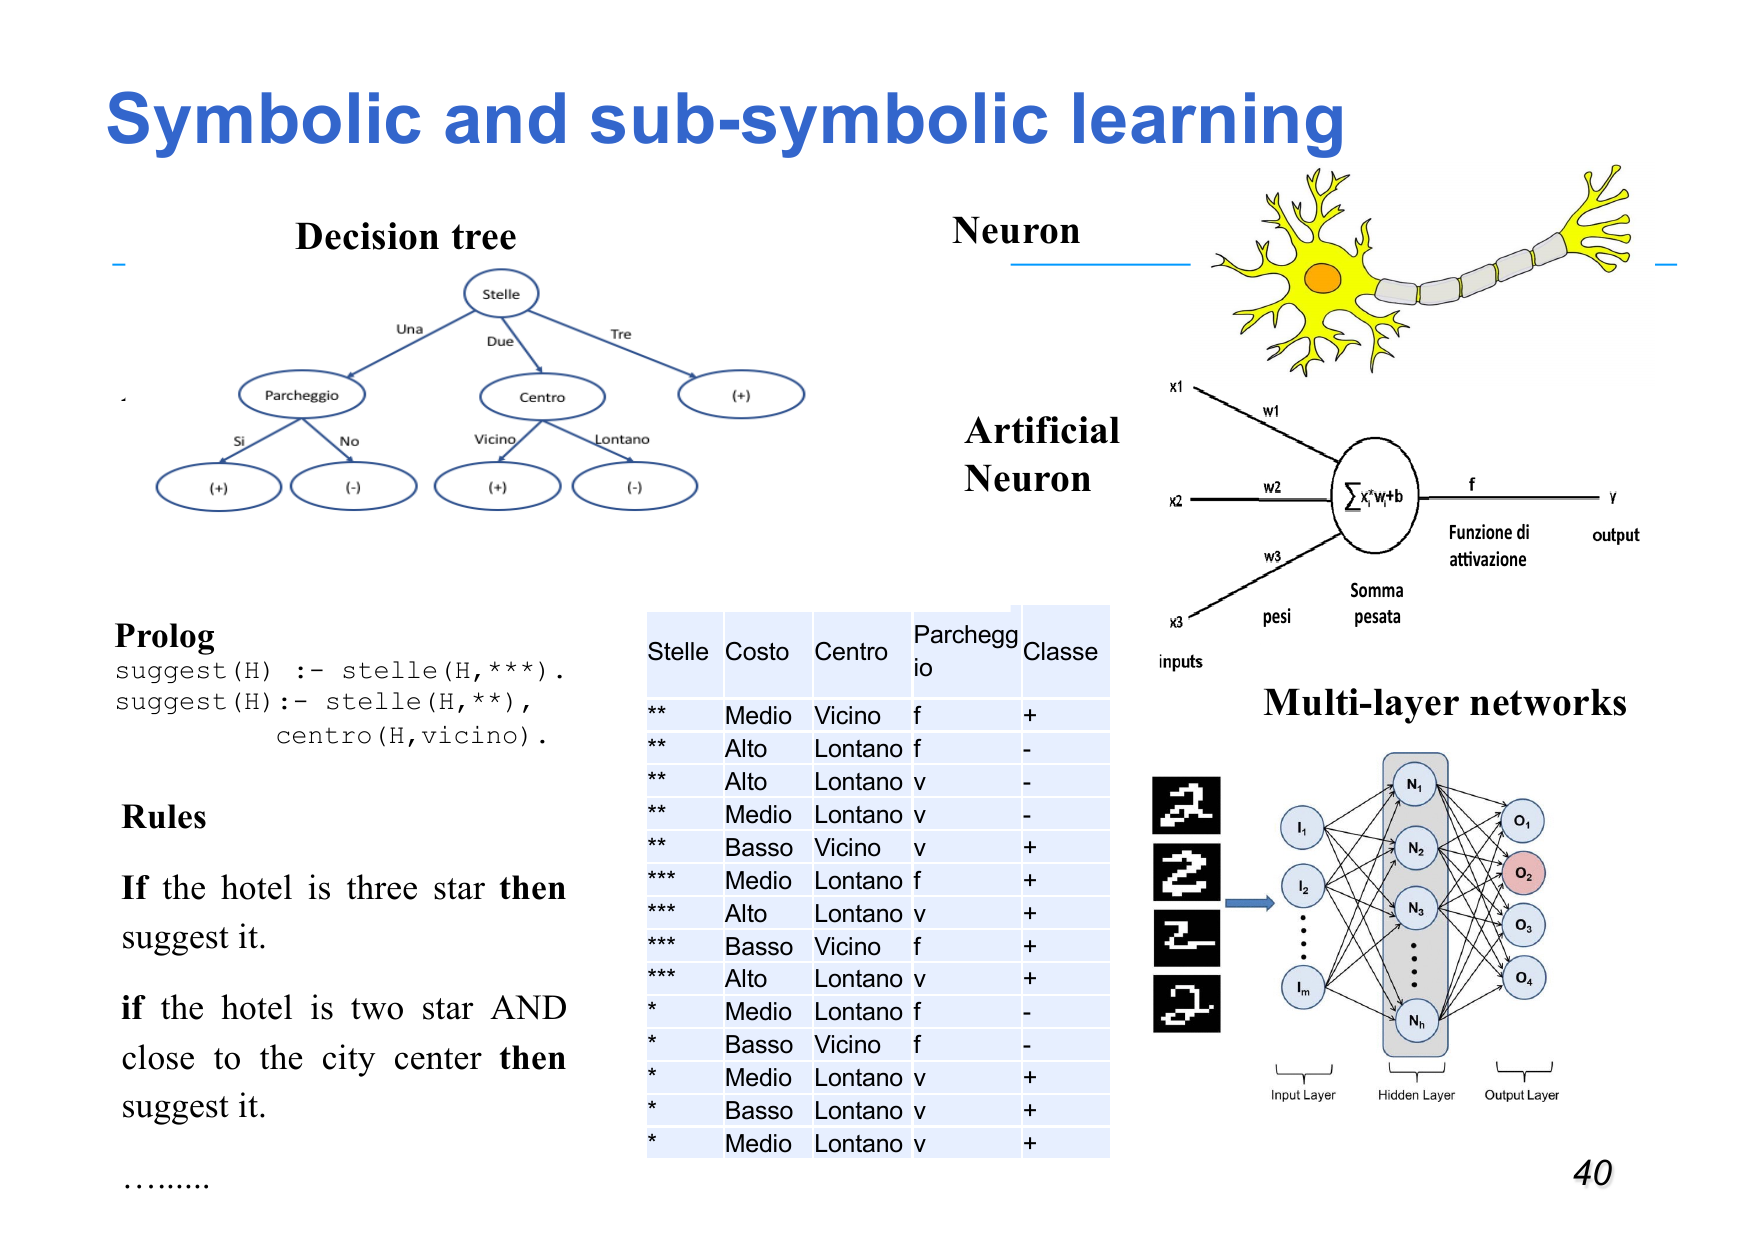
\includegraphics[width=0.9\textwidth]{img/simbolico-subsimbolico.png}
  \caption{Due mondi a confronto: albero di decisione (e regole Prolog) contro
  neurone artificiale e reti multi-livello.}
\end{figure}

\subsection{Apprendimento simbolico: alberi di decisione (ID3, C4.5)}

\begin{Example}{Training set degli hotel}{}
  \begin{center}
  \begin{tabular}{|l|l|l|l|c|}
    \hline
    \textbf{Stelle} & \textbf{Costo} & \textbf{Centro} & \textbf{Parcheggio}
      & \textbf{Classe}\\
    \hline
    ** & Medio & Vicino & f & $+$\\
    ** & Alto & Lontano & f & $-$\\
    ** & Alto & Lontano & v & $-$\\
    ** & Medio & Lontano & v & $-$\\
    ** & Basso & Vicino & v & $+$\\
    *** & Medio & Lontano & f & $+$\\
    *** & Alto & Lontano & v & $+$\\
    *** & Basso & Vicino & f & $+$\\
    *** & Alto & Lontano & v & $+$\\
    * & Medio & Lontano & f & $-$\\
    * & Basso & Vicino & f & $-$\\
    * & Medio & Lontano & v & $+$\\
    * & Basso & Lontano & v & $+$\\
    * & Medio & Lontano & v & $+$\\
    \hline
  \end{tabular}
  \end{center}

  L'albero di decisione appreso si traduce in \textbf{regole leggibili}:
  \begin{itemize}
    \item se l'hotel è a tre stelle allora suggeriscilo;
    \item se l'hotel è a due stelle \textbf{AND} è vicino al centro allora
      suggeriscilo;
    \item \dots
  \end{itemize}
  che in Prolog diventano:
\begin{lstlisting}
suggest(H) :- stelle(H,***).
suggest(H) :- stelle(H,**), centro(H,vicino).
\end{lstlisting}
\end{Example}

\begin{figure}[H]
  \centering
  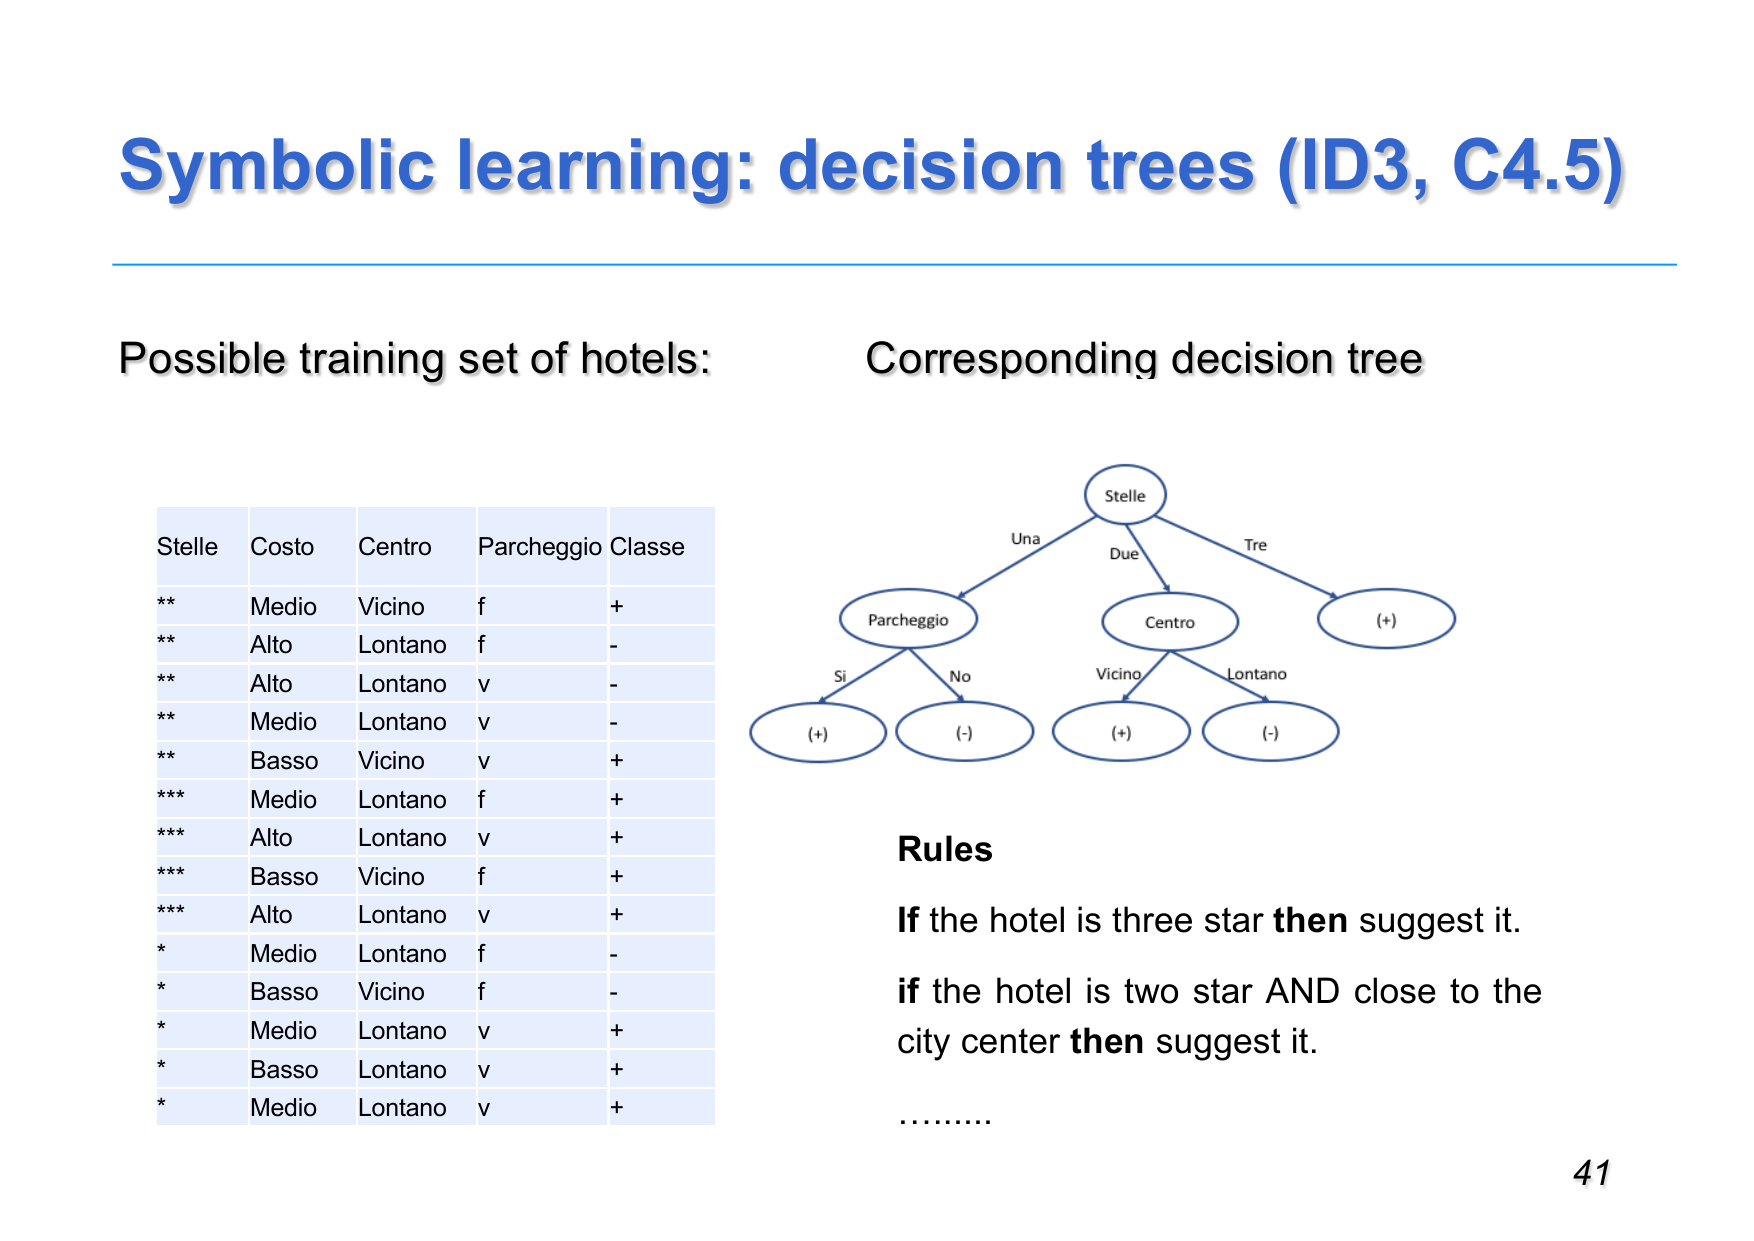
\includegraphics[width=0.85\textwidth]{img/albero-decisione.png}
  \caption{Training set degli hotel e albero di decisione corrispondente.}
\end{figure}

\nt{
  Il punto di forza dell'approccio simbolico è qui evidente: il modello appreso è
  \textbf{ispezionabile} e traducibile in regole logiche. È esattamente ciò che si
  perde passando alle reti neurali.
}

\subsection{Il neurone artificiale}

L'idea è \textbf{simulare direttamente il funzionamento del cervello} in un
calcolatore, e costruire una macchina intelligente a partire da neuroni artificiali.
Il primo modello matematico di neurone artificiale, ispirato ai neuroni biologici, è
stato proposto nel \textbf{1943} da \textbf{McCulloch e Pitts}.

\dfn{Neurone artificiale}{
  Un neurone riceve un insieme di \textbf{input}, ne fa una \textbf{somma pesata} e
  poi applica una \textbf{funzione di attivazione} per calcolare l'output.

  L'output è controllato dalla funzione di attivazione: ogni neurone è
  \textbf{attivo} solo se il suo input supera una certa \textbf{soglia}.
}

\begin{figure}[H]
  \centering
  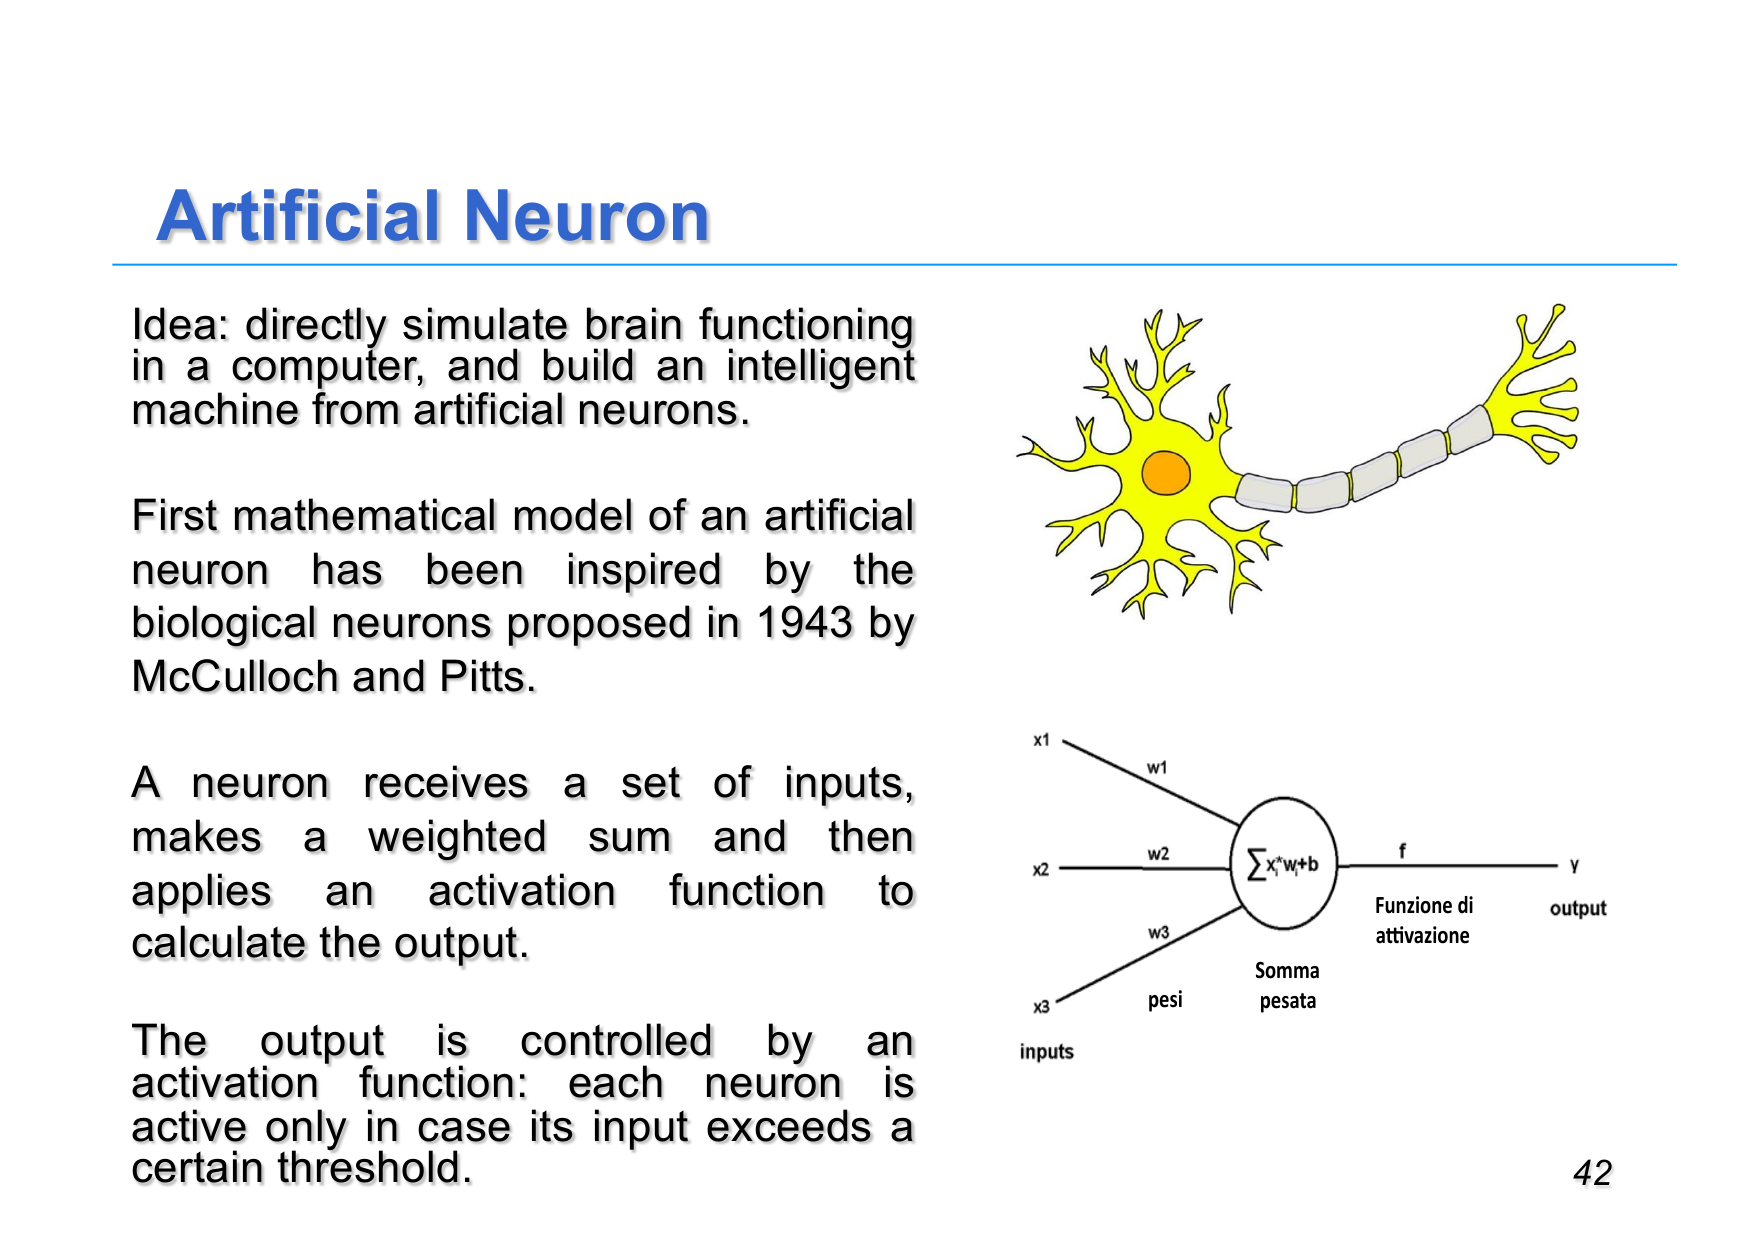
\includegraphics[width=0.8\textwidth]{img/neurone-artificiale.png}
  \caption{Neurone biologico e neurone artificiale: pesi, somma pesata, funzione di
  attivazione.}
\end{figure}

\subsection{Il percettrone a due input}

\dfn{Percettrone}{
  Con due input $x_1, x_2$, pesi $w_1, w_2$ e soglia $\theta$:
  \[
    y = H_S\!\left(w_1 x_1 + w_2 x_2 - \theta\right)
  \]
  dove $H_S$ è la funzione a gradino (Heaviside). I pattern appartenenti alla classe
  sono quelli tali che
  \[
    w_1 x_1 + w_2 x_2 - \theta > 0 .
  \]
}

\begin{figure}[H]
  \centering
  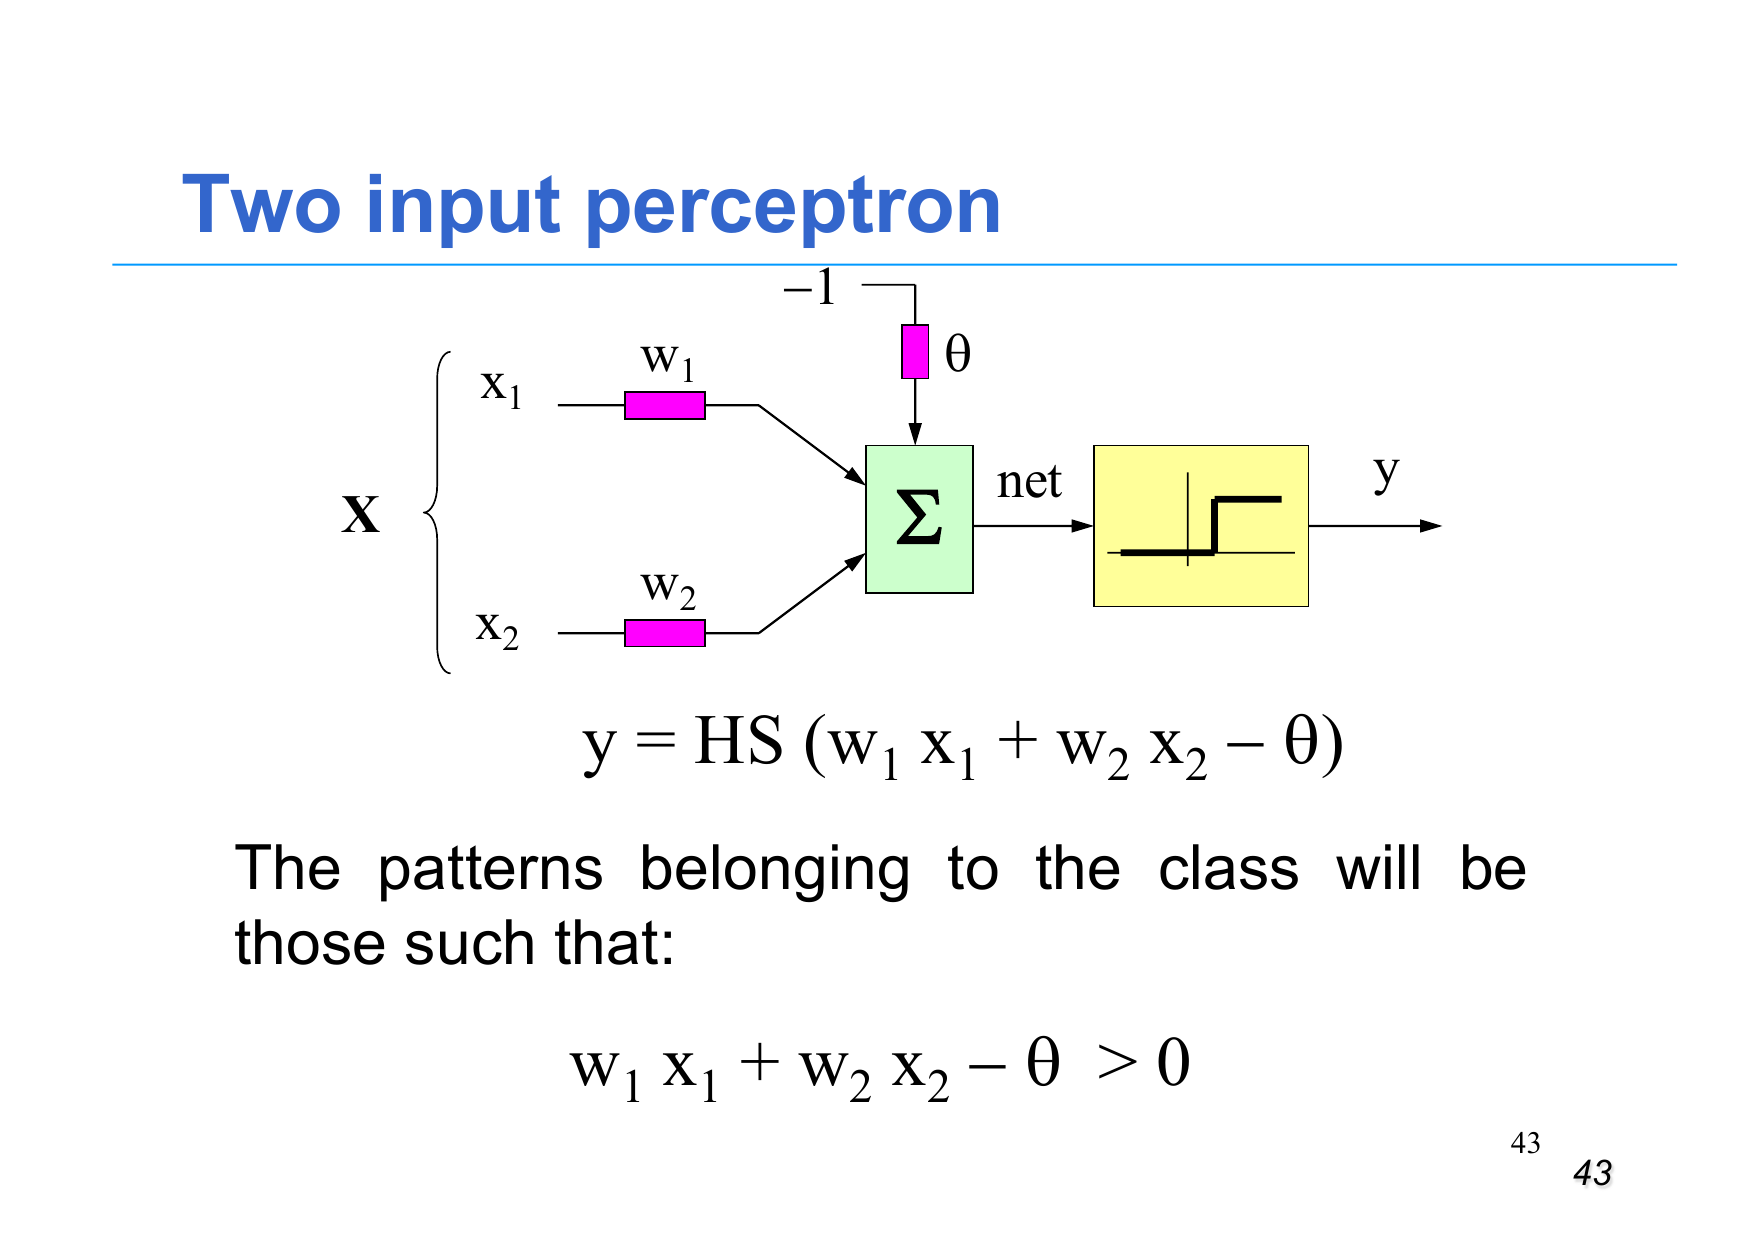
\includegraphics[width=0.6\textwidth]{img/percettrone.png}
  \caption{Percettrone a due input.}
\end{figure}

\mprop{Separazione lineare dello spazio di input}{
  La condizione $w_1 x_1 + w_2 x_2 - \theta > 0$ si riscrive come
  \[
    x_2 > -\frac{w_1}{w_2}\, x_1 + \frac{\theta}{w_2}
  \]
  che è il semipiano sopra una \textbf{retta}: il percettrone realizza dunque una
  \textbf{separazione lineare} dello spazio di input. La retta interseca gli assi in
  $\theta/w_1$ e $\theta/w_2$.
}

\begin{figure}[H]
  \centering
  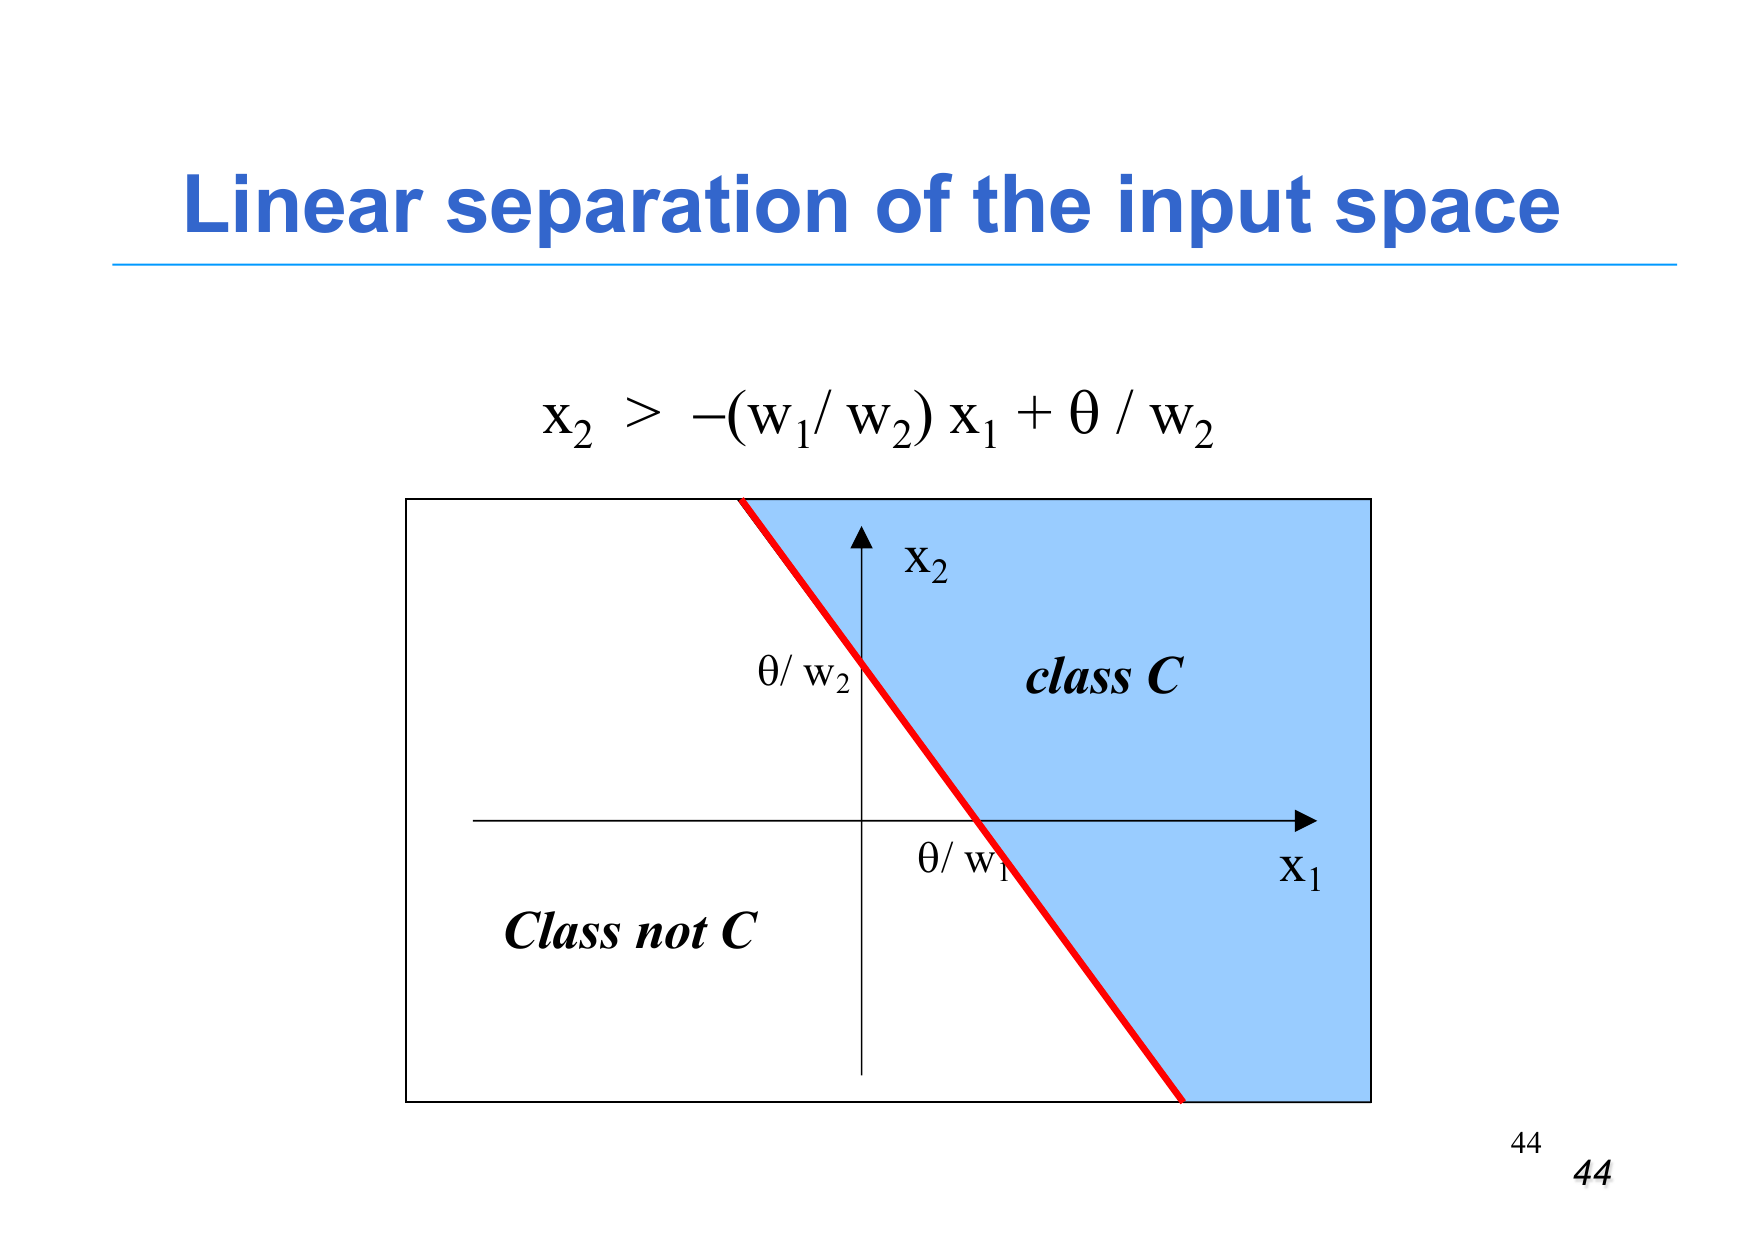
\includegraphics[width=0.65\textwidth]{img/separazione-lineare.png}
  \caption{La retta di separazione divide la classe $C$ dalla classe non-$C$.}
\end{figure}

\ex{Apprendere la porta AND}{
  Con la regola di aggiornamento $\Delta w = \eta\,\delta\,x$ si arriva ai pesi
  \[
    w_1 = 0.5, \qquad w_2 = 1, \qquad \theta = 1
  \]
  che separano il punto $(1,1)$ (unico output positivo dell'AND) da $(0,0)$, $(0,1)$
  e $(1,0)$.
}

\begin{figure}[H]
  \centering
  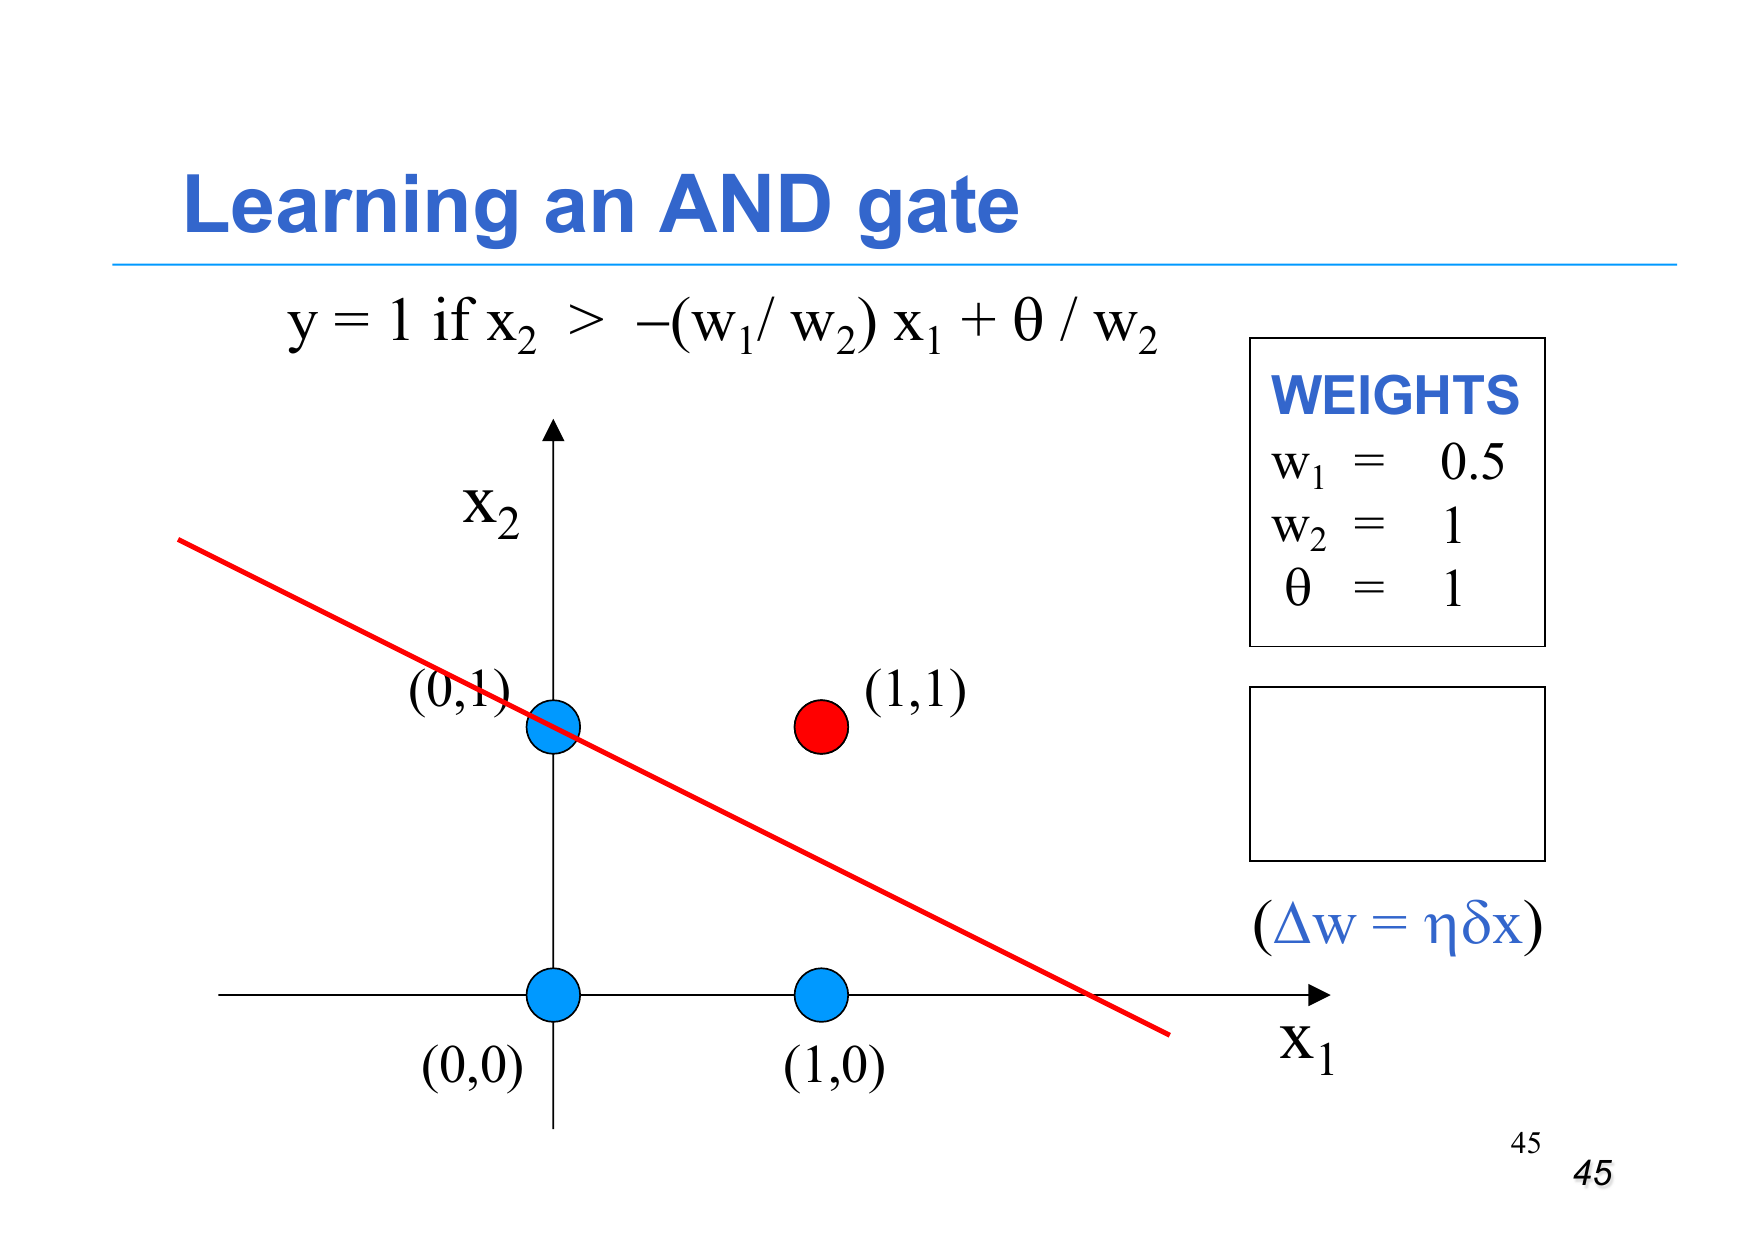
\includegraphics[width=0.6\textwidth]{img/and-gate.png}
  \caption{Apprendimento della porta AND: retta di separazione e pesi.}
\end{figure}

\subsection{Reti neurali multi-livello}

Per rappresentare concetti più complessi occorre costruire \textbf{reti di neuroni}:
architetture \textbf{multi-livello} (reti \emph{forward} o \emph{feed-forward}) e
nuovi algoritmi di apprendimento.

\nt{
  È un approccio \textbf{significativamente diverso} da quello simbolico: la
  conoscenza non è esplicita, ma è \textbf{insita nella struttura della rete e nei
  pesi delle connessioni}.
}

\begin{figure}[H]
  \centering
  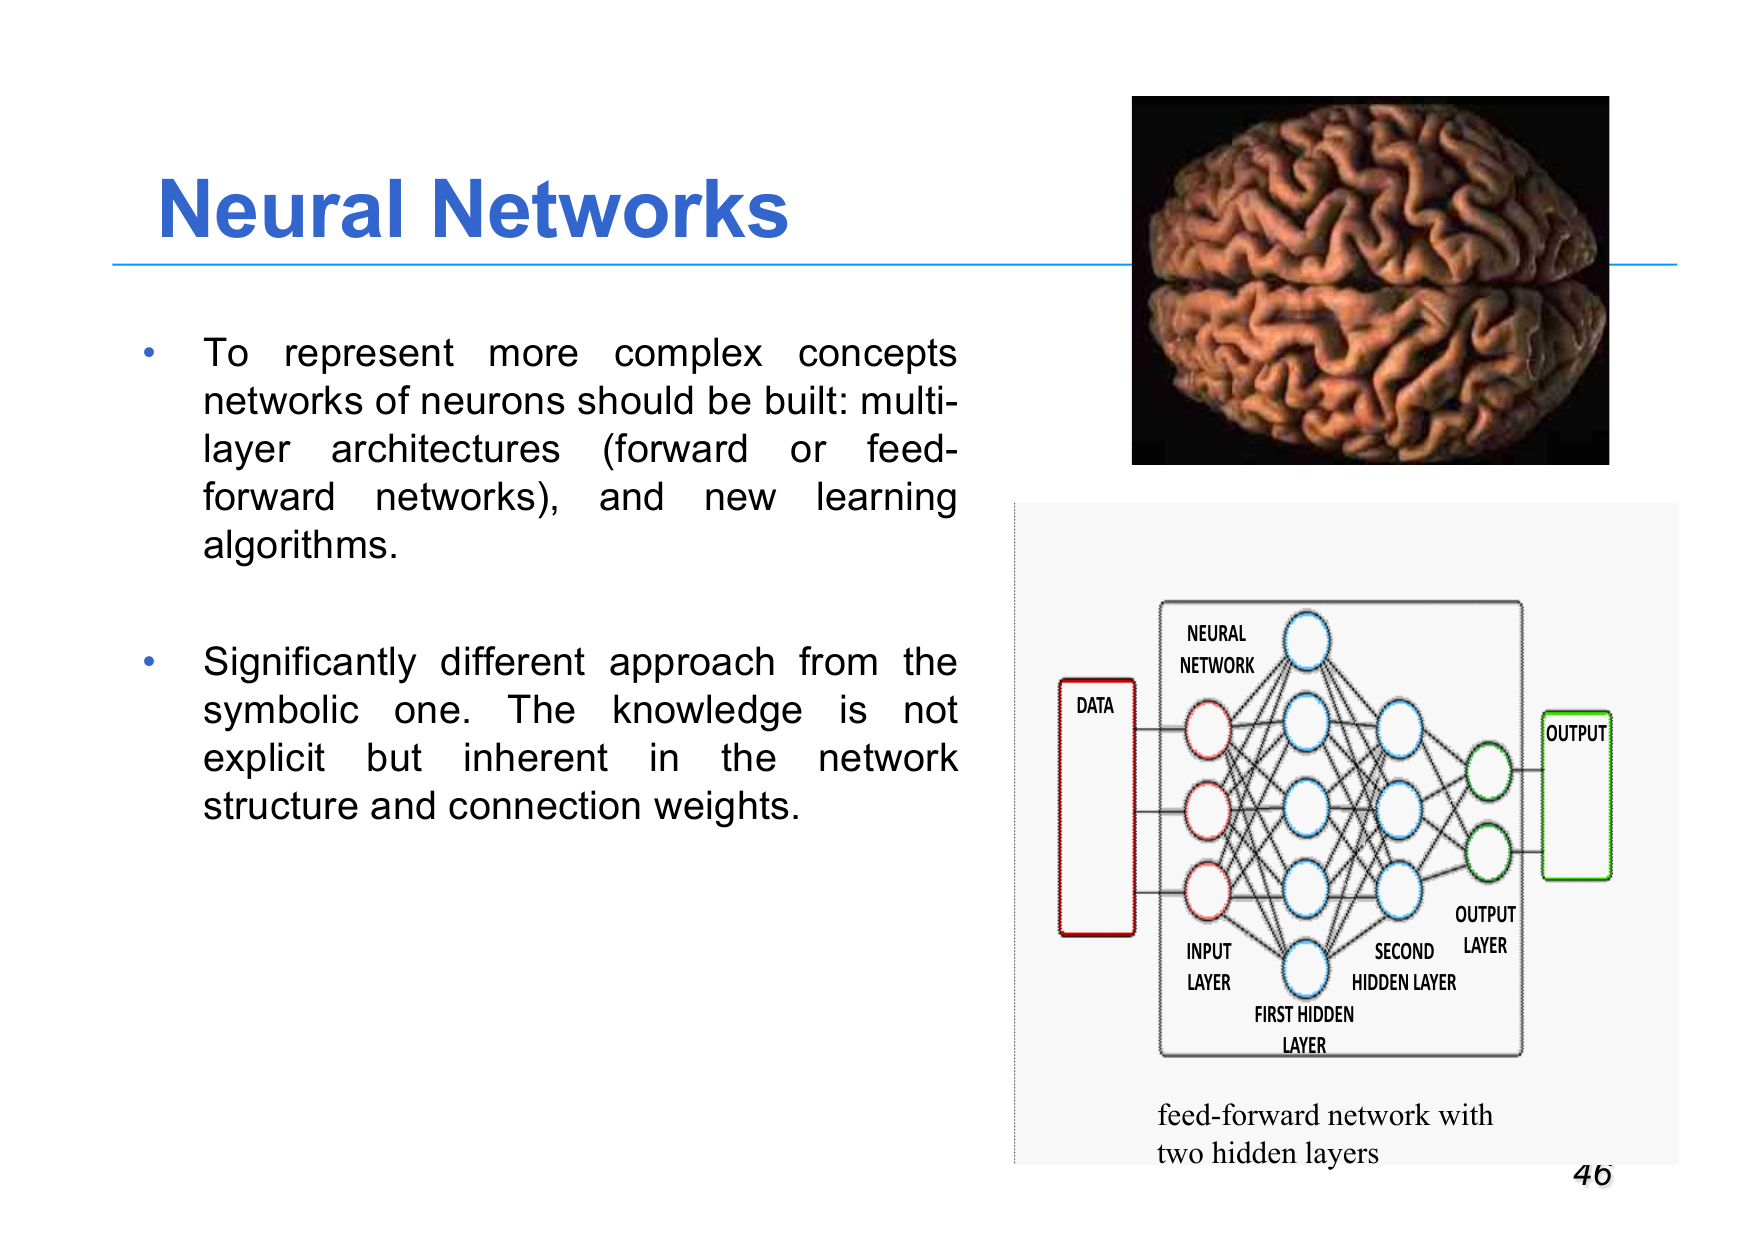
\includegraphics[width=0.85\textwidth]{img/rete-feedforward.png}
  \caption{Rete feed-forward con due hidden layer.}
\end{figure}

\mprop{Potere espressivo in funzione dei livelli}{
  \begin{itemize}
    \item \textbf{Reti a due livelli} (percettrone): separano solo regioni
      \textbf{linearmente separabili};
    \item \textbf{Reti a tre livelli}: separano \textbf{regioni convesse}, con
      $\text{numero di lati} \leq \text{numero di neuroni nascosti}$;
    \item \textbf{Reti a quattro livelli}: separano regioni di \textbf{qualsiasi
      forma}.
  \end{itemize}
}

\begin{figure}[H]
  \centering
  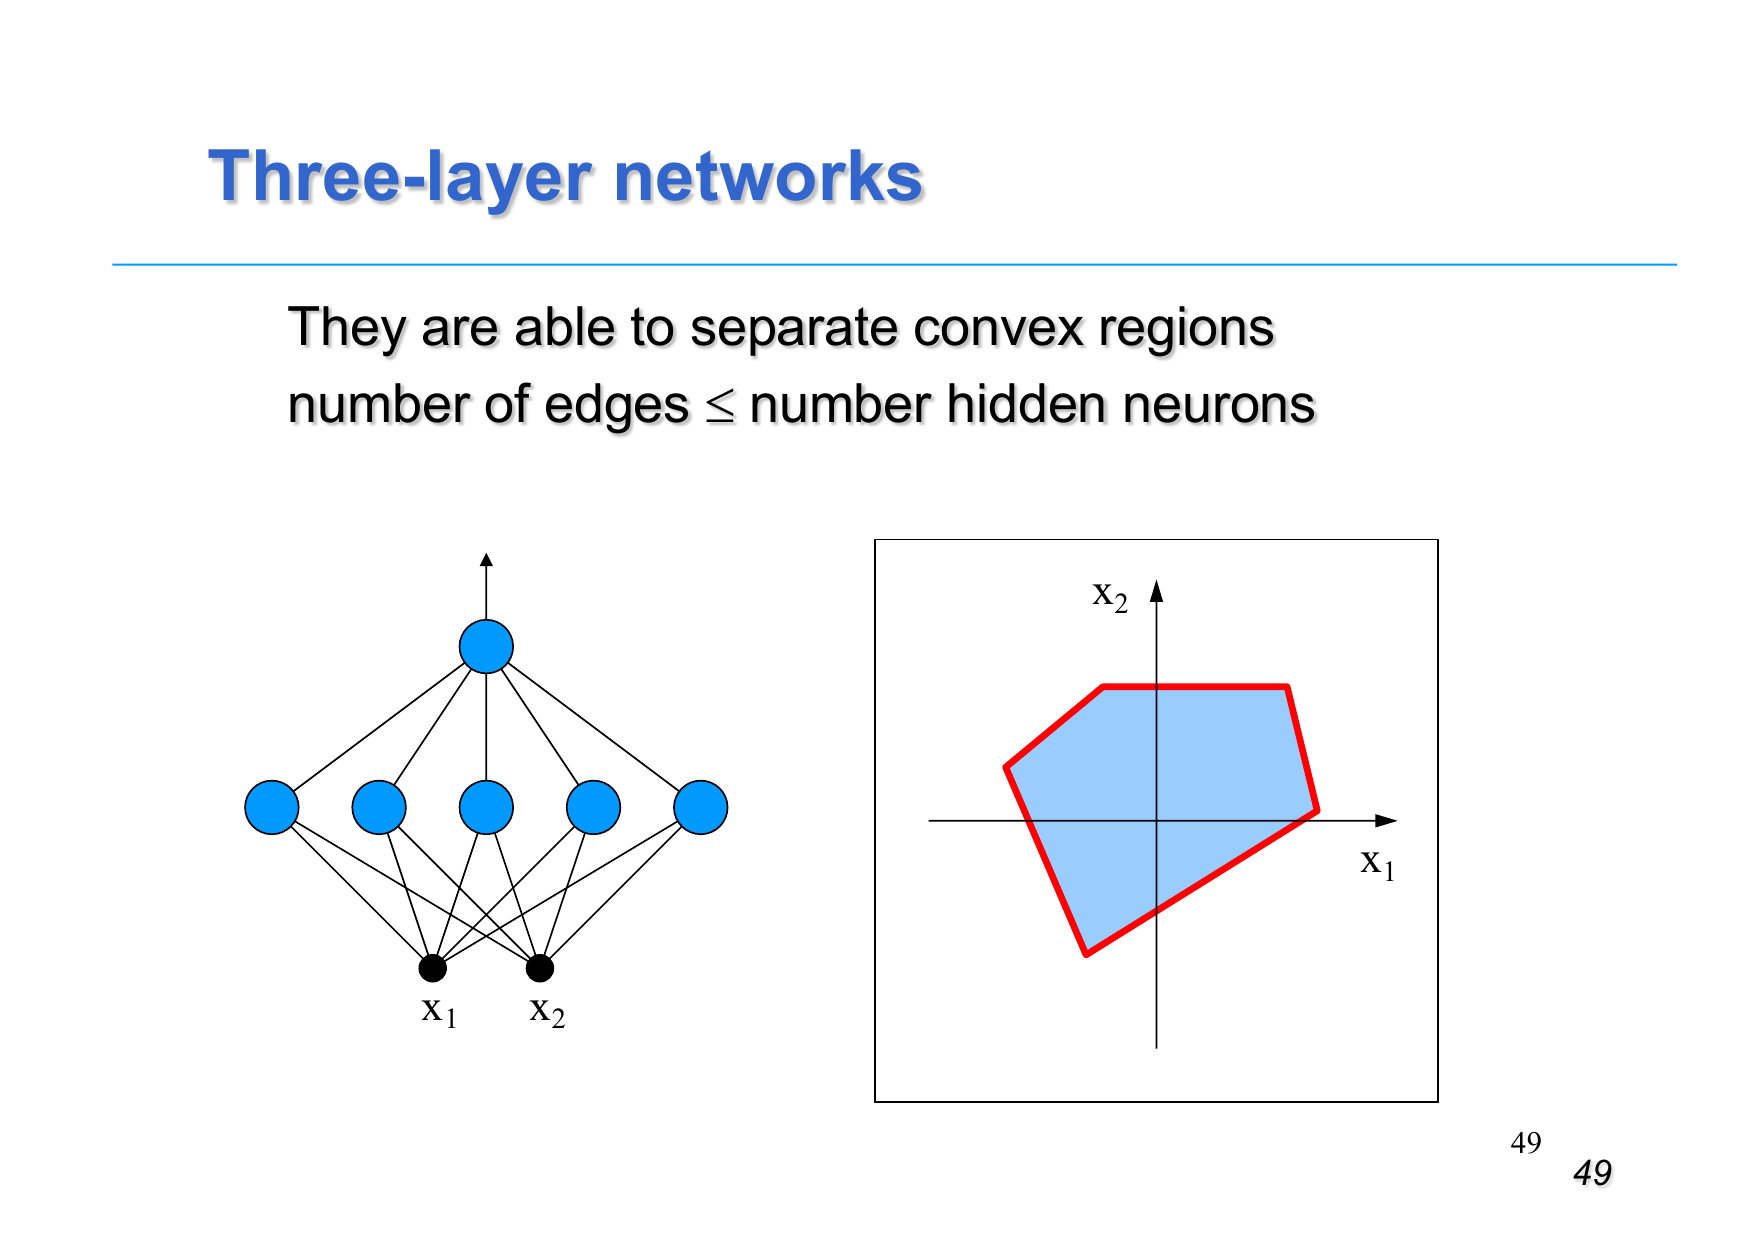
\includegraphics[width=0.48\textwidth]{img/regioni-convesse.png}
  \hfill
  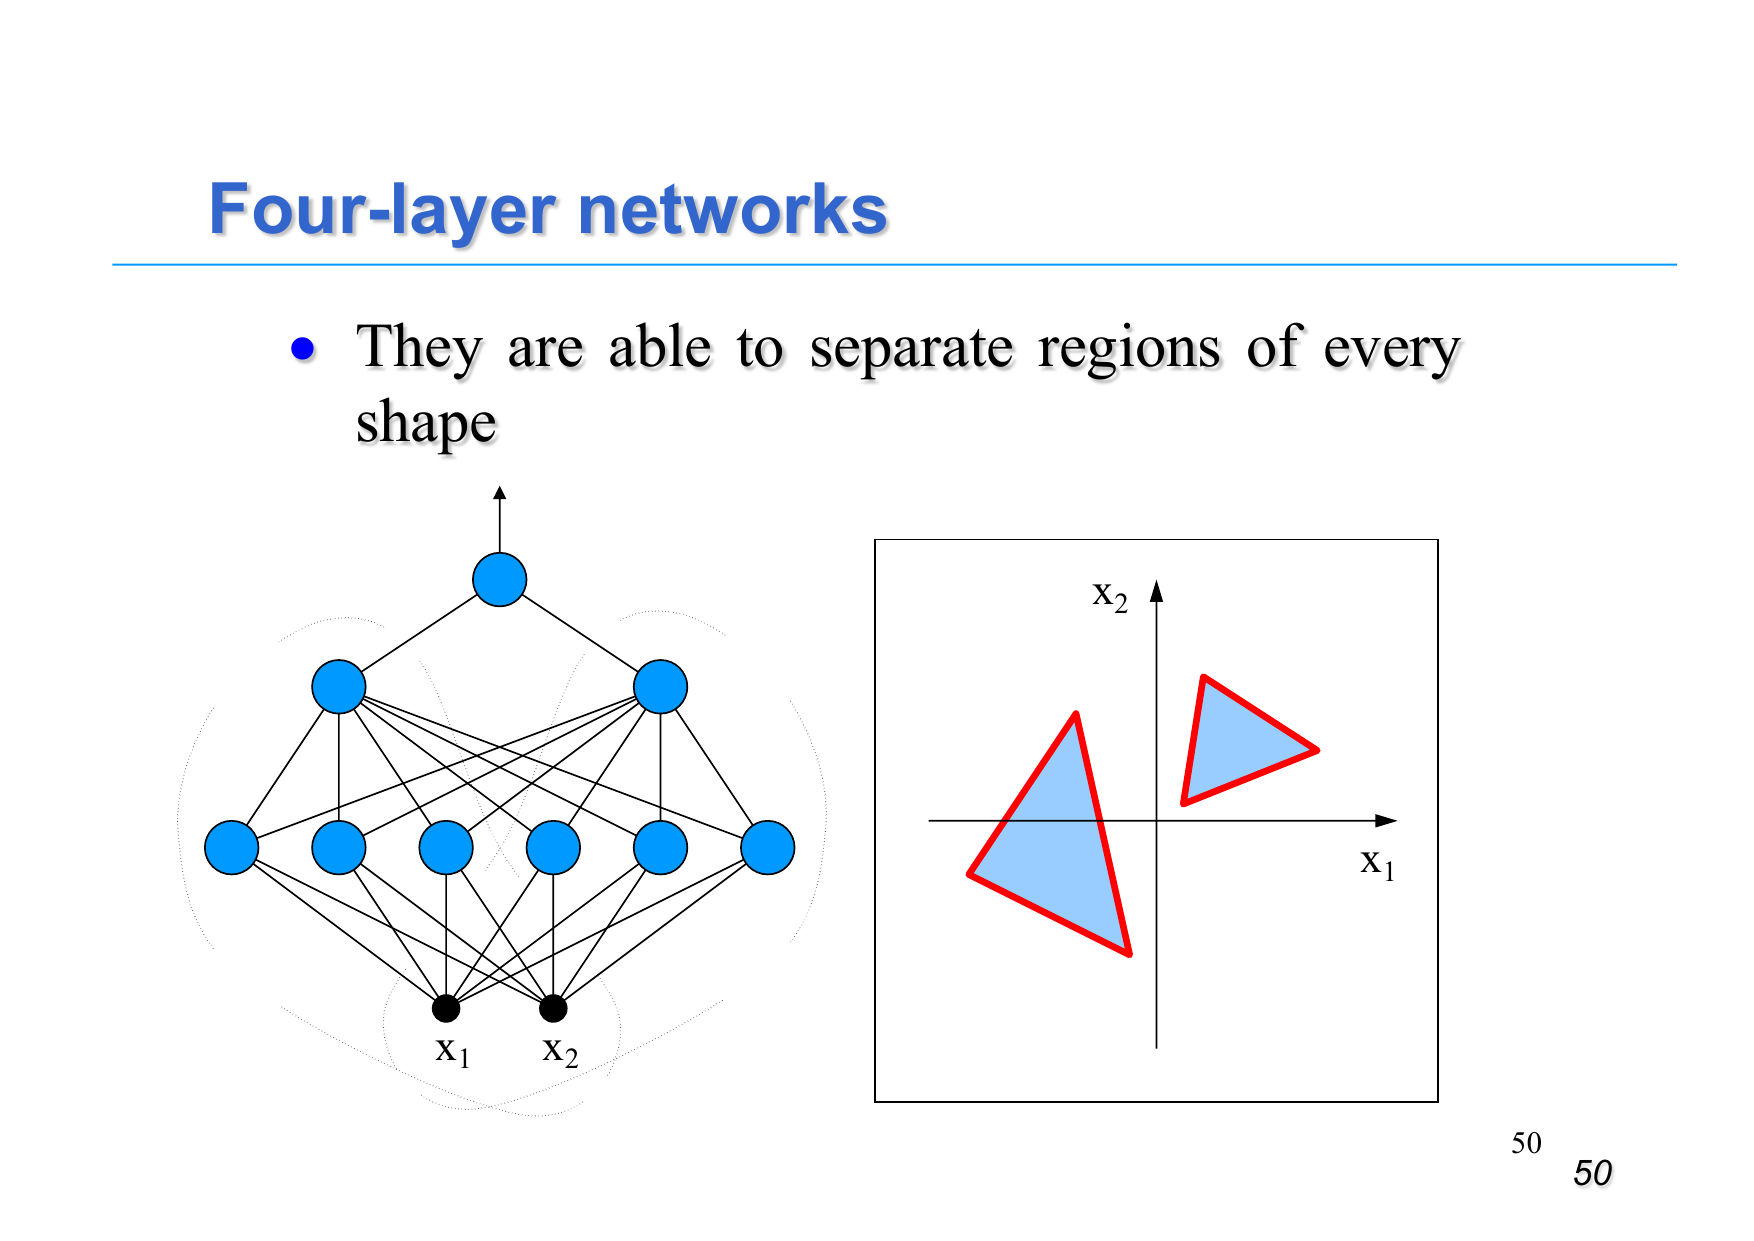
\includegraphics[width=0.48\textwidth]{img/regioni-qualsiasi.png}
  \caption{A sinistra: reti a tre livelli e regioni convesse. A destra: reti a
  quattro livelli e regioni di forma arbitraria.}
\end{figure}

\thm{Teorema di approssimazione universale}{
  Una rete \textbf{feed-forward} con \textbf{un solo hidden layer} e un
  \textbf{numero finito di neuroni} può approssimare \textbf{qualsiasi funzione
  continua} con l'accuratezza desiderata.
}

\nt{
  Teoria interessante, ma non dice \textbf{nulla} su come configurare la rete né su
  come applicare gli algoritmi di apprendimento per ottenere una buona
  approssimazione. Quali funzioni di output? Quanti neuroni? Quanti livelli?
}

Dagli anni '80 sono stati progettati modelli di neurone artificiale più complessi e
dettagliati, con diverse funzioni \textbf{non lineari} (per esempio la
\textbf{sigmoide}); sono state individuate varie \textbf{architetture} e sviluppati
algoritmi di apprendimento più sofisticati.

\section{Deep Neural Networks e Deep Learning}

\dfn{Deep Learning}{
  Modelli e algoritmi che usano reti neurali con \textbf{molti neuroni} e
  \textbf{molti livelli}. Riescono ad apprendere funzioni complesse, cercando di
  individuare i dati più rilevanti.
}

\mprop{Caratteristiche delle DNN}{
  \begin{itemize}
    \item le DNN più usate hanno un numero molto elevato di livelli (anche qualche
      \textbf{centinaio});
    \item il processo di \textbf{training è computazionalmente costoso};
    \item gli algoritmi supervisionati attualmente ottengono buone prestazioni con
      circa \textbf{5\,000 esempi per categoria} e \textbf{superano gli umani con
      10 milioni di esempi};
    \item \textbf{non} è una ``simulazione'' del cervello, che ha molti più neuroni e
      una struttura ben più complessa. Con un ulteriore sviluppo della potenza di
      calcolo si avrà un numero di neuroni confrontabile con quello umano
      nel \textbf{2050}.
  \end{itemize}
  \hfill \footnotesize{Da: I.~Goodfellow, Y.~Bengio, A.~Courville,
  \emph{Deep Learning}, MIT Press, 2016.}
}

\nt{
  Nel Deep Learning i concetti sono appresi attraverso una \textbf{gerarchia di
  feature}, dalle più semplici alle più astratte e complesse. La rappresentazione è
  \textbf{implicitamente distribuita} nei diversi livelli.
}

\begin{figure}[H]
  \centering
  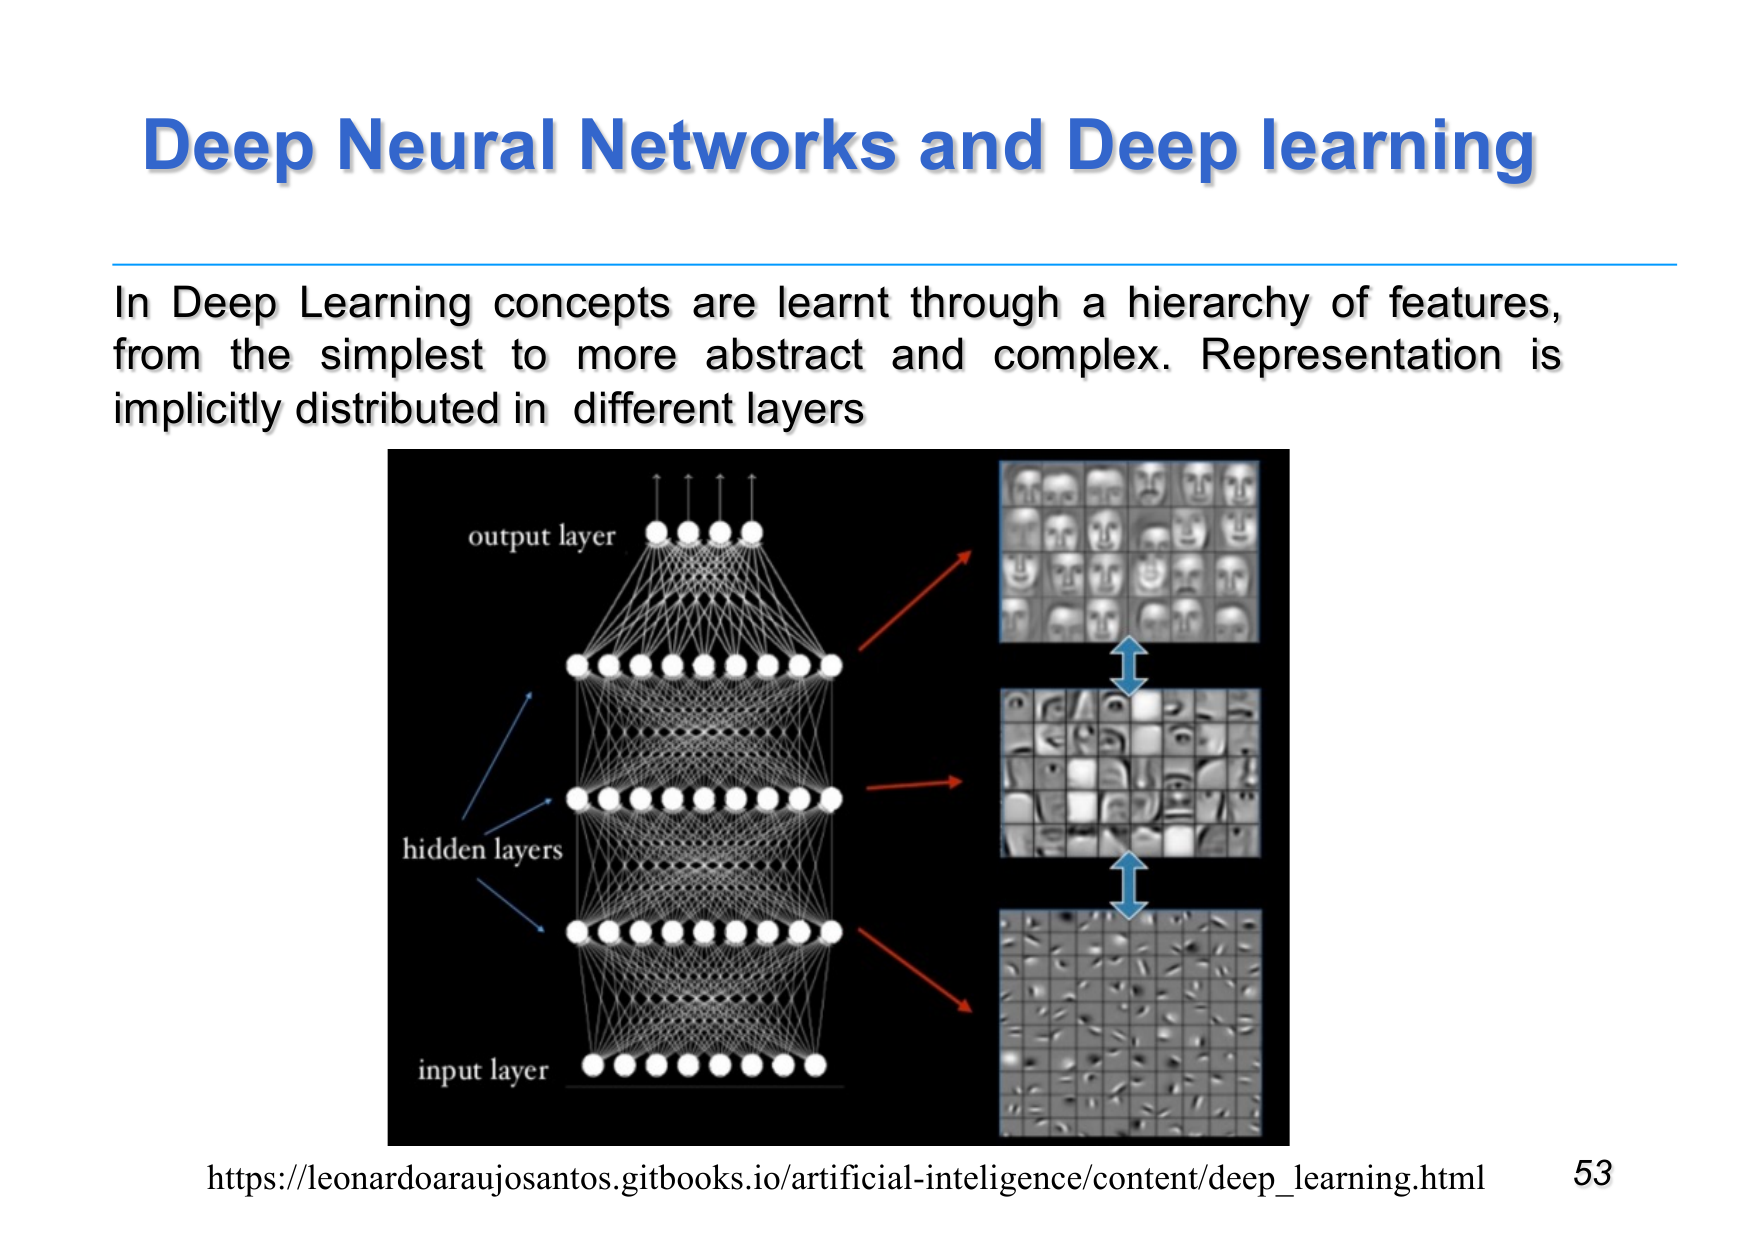
\includegraphics[width=0.8\textwidth]{img/deep-features.png}
  \caption{Gerarchia di feature nel deep learning: dai bordi alle parti agli
  oggetti.}
\end{figure}

\section{Foundation Models}

\dfn{Foundation model}{
  Modelli su \textbf{larga scala} pre-addestrati su dati ampi e diversificati, poi
  \textbf{adattati} per alimentare innumerevoli applicazioni a valle. Sono
  il ``base layer'' dell'IA moderna.
}

\mprop{Tre caratteristiche dei foundation model}{
  \begin{enumerate}
    \item \textbf{Trained at Massive Scale} -- apprendono da dataset ampi e
      diversificati che spaziano tra testo, codice, immagini e altro;
    \item \textbf{Transformer Architecture} -- la \emph{self-attention} permette al
      modello di pesare le relazioni lungo sequenze di input molto lunghe;
    \item \textbf{General-Purpose by Design} -- un unico modello pre-addestrato si
      trasferisce a molti task tramite \textbf{fine-tuning} o \textbf{prompting}.
  \end{enumerate}
}

\begin{center}
\begin{tabular}{p{0.45\textwidth}|p{0.45\textwidth}}
  \textbf{Traditional AI} & \textbf{Foundation Models}\\
  \hline
  costruita per un task specifico & pre-addestrati una volta su dati ampi\\
  addestrata da zero ogni volta & adattati via fine-tuning o prompting\\
  richiede grandi dataset etichettati per ogni task
    & riusati su molti task e domini\\
  trasferimento limitato a nuovi domini & capaci di uso \emph{few-shot} o
    \emph{zero-shot}\\
\end{tabular}
\end{center}

\nt{
  Esempi: GPT, Claude, Gemini, Llama, Stable Diffusion.
}

\section{Agentic AI}

\dfn{Sistema agentico}{
  I sistemi agentici \textbf{ragionano su un obiettivo}, \textbf{pianificano più
  passi}, \textbf{usano strumenti} e \textbf{si correggono} sulla base di ciò che
  osservano. Non si limitano a rispondere: \emph{agiscono}.
}

\mprop{Il ciclo dell'agente}{
  \begin{enumerate}
    \item \textbf{Perceive / Observe} -- raccoglie contesto dall'ambiente, dagli
      strumenti e dai passi precedenti;
    \item \textbf{Plan} -- scompone l'obiettivo in una sequenza di sotto-task e
      decisioni;
    \item \textbf{Act} -- chiama tool, API o altri sistemi per compiere azioni reali;
    \item \textbf{Reflect} -- valuta i risultati e adatta il piano, tornando al passo 1.
  \end{enumerate}
  Applicazioni tipiche: \emph{coding agent}, assistenti di ricerca, automazione di
  workflow, agenti di customer support.
}

\begin{figure}[H]
  \centering
  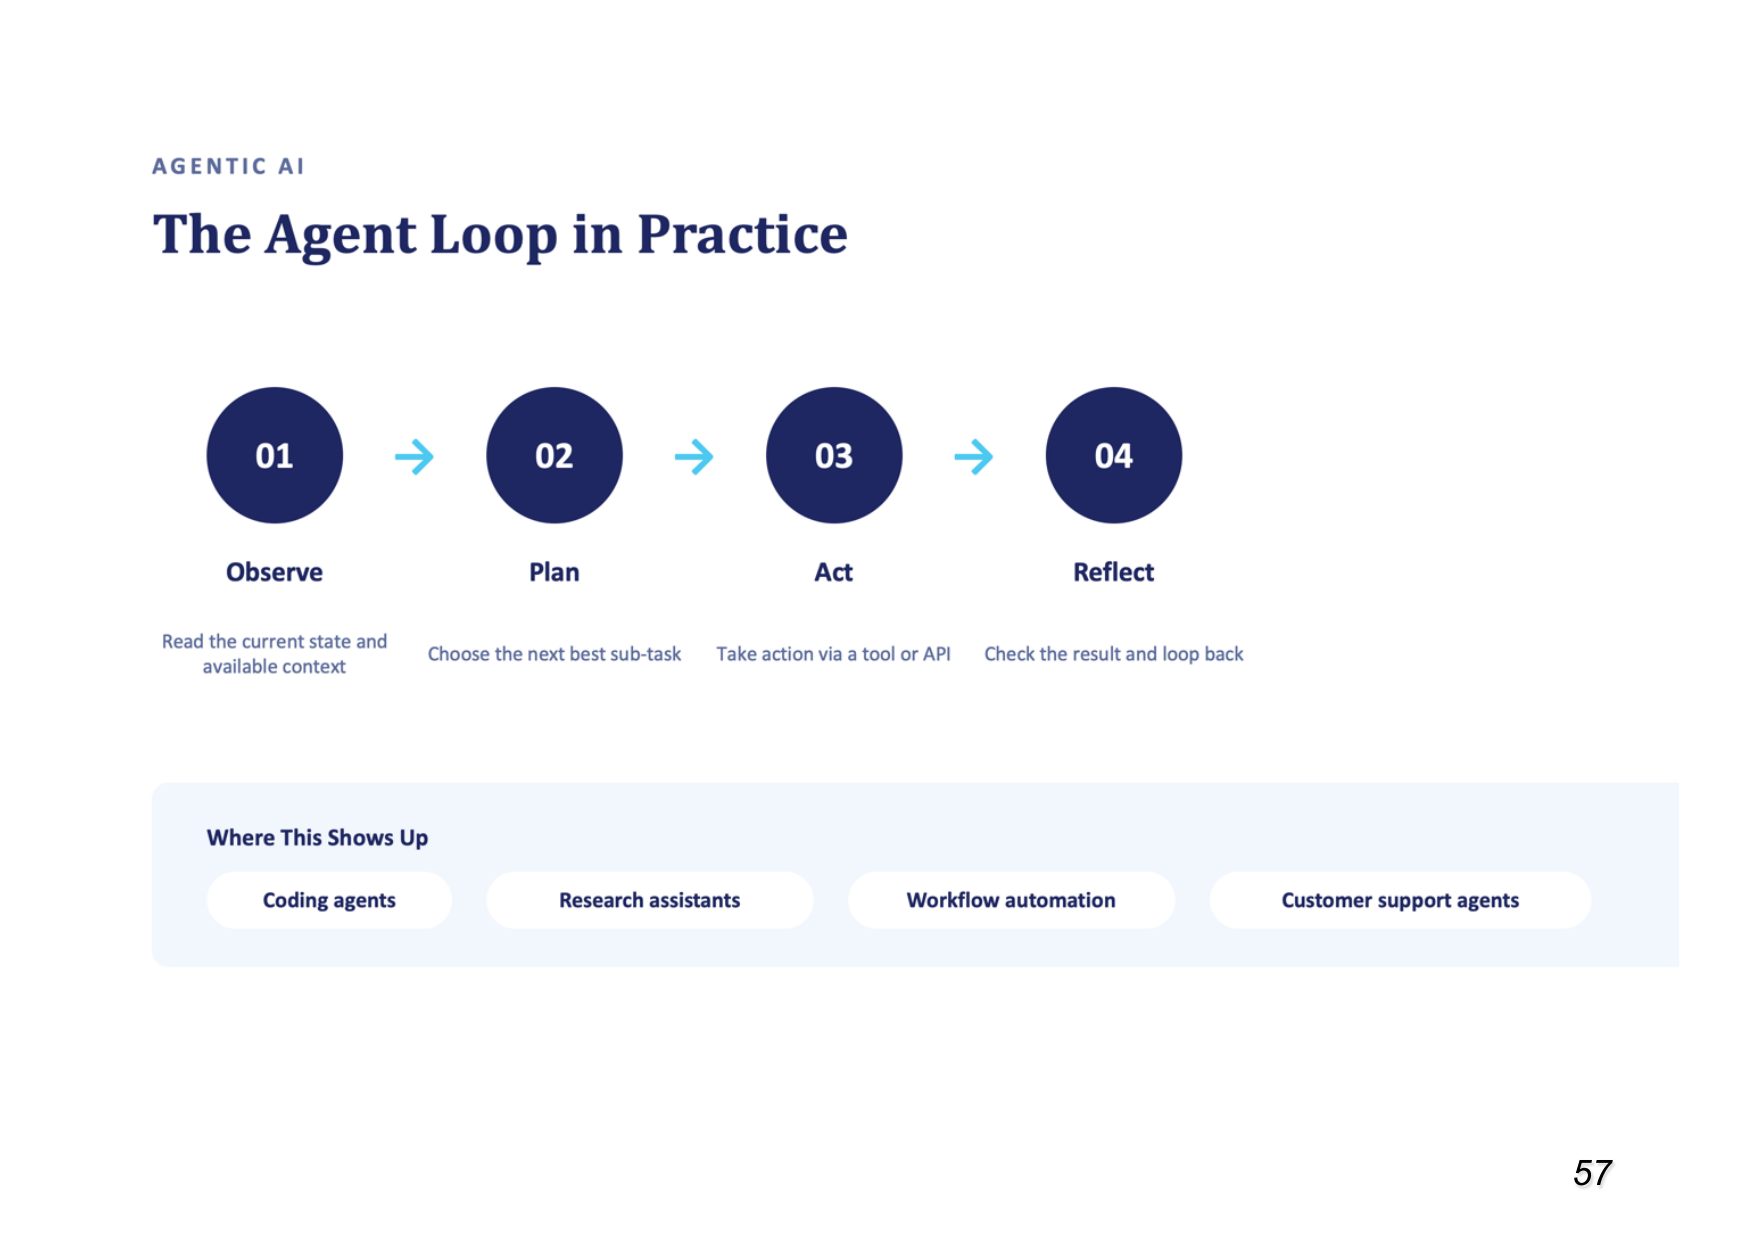
\includegraphics[width=0.9\textwidth]{img/agent-loop.png}
  \caption{Il loop dell'agente: Observe $\to$ Plan $\to$ Act $\to$ Reflect.}
\end{figure}

\nt{
  Il ciclo agentico è, a ben vedere, una riedizione del \textbf{planning automatico}
  classico (stato iniziale, azioni, goal) in cui il motore di pianificazione è un
  foundation model invece di un planner simbolico.
}

\section{Automated Planning}

\dfn{Planning automatico}{
  Il planning automatico è un'importante attività di problem solving che consiste nel
  \textbf{sintetizzare una sequenza di azioni} eseguite da un agente, che porta da
  uno \textbf{stato iniziale} del mondo a un dato \textbf{stato obiettivo} (goal).

  \textbf{Dati:}
  \begin{itemize}
    \item uno \textbf{stato iniziale};
    \item un insieme di \textbf{azioni} eseguibili;
    \item uno \textbf{stato da raggiungere} (goal).
  \end{itemize}
  \textbf{Trovare:} un \textbf{piano}, cioè un insieme di azioni parzialmente o
  totalmente ordinato, necessario a raggiungere il goal dallo stato iniziale.
}

\dfn{Planner}{
  Un planner automatico è un agente intelligente che opera in un certo dominio,
  descritto da:
  \begin{enumerate}
    \item una \textbf{rappresentazione dello stato iniziale};
    \item una \textbf{rappresentazione del goal};
    \item una \textbf{descrizione formale delle azioni} eseguibili (dette anche
      \textbf{operatori}) in termini di \textbf{precondizioni} ed \textbf{effetti}.
  \end{enumerate}
  Definisce dinamicamente il piano di azioni necessario a raggiungere il goal dallo
  stato iniziale.
}

\subsection{Esempio: il mondo dei blocchi}

\ex{Operatori del block world}{
  \textbf{STACK(X,Y)} -- impila $X$ su $Y$
  \begin{itemize}
    \item \textbf{IF}: \texttt{holding(X)} $\wedge$ \texttt{clear(Y)}
    \item \textbf{THEN}: \texttt{handempty} $\wedge$ \texttt{clear(X)} $\wedge$
      \texttt{on(X,Y)}
  \end{itemize}

  \textbf{UNSTACK(X,Y)} -- disimpila $X$ da $Y$
  \begin{itemize}
    \item \textbf{IF}: \texttt{handempty} $\wedge$ \texttt{clear(X)} $\wedge$
      \texttt{on(X,Y)}
    \item \textbf{THEN}: \texttt{holding(X)} $\wedge$ \texttt{clear(Y)}
  \end{itemize}

  \textbf{PICKUP(X)} -- prendi $X$ dal tavolo
  \begin{itemize}
    \item \textbf{IF}: \texttt{ontable(X)} $\wedge$ \texttt{clear(X)} $\wedge$
      \texttt{handempty}
    \item \textbf{THEN}: \texttt{holding(X)}
  \end{itemize}

  \textbf{PUTDOWN(X)} -- posa $X$ sul tavolo
  \begin{itemize}
    \item \textbf{IF}: \texttt{holding(X)}
    \item \textbf{THEN}: \texttt{ontable(X)} $\wedge$ \texttt{clear(X)} $\wedge$
      \texttt{handempty}
  \end{itemize}
}

\nt{
  Si noti la struttura \textbf{precondizione $\to$ effetto} di ogni operatore:
  è esattamente la forma richiesta dalla definizione di planner. Le azioni sono
  duali a coppie (STACK/UNSTACK, PICKUP/PUTDOWN).
}

\subsection{Tecniche di planning}

\begin{itemize}
  \item \textbf{Deductive planning} / \textbf{planning as search} / \textbf{linear
    planning} (trattati in \emph{Foundations of AI});
  \item \textbf{Nonlinear planning}, in particolare \textbf{Partial Order Planning}
    (POP);
  \item \textbf{Hierarchical planning};
  \item \textbf{Conditional planning};
  \item \textbf{Graph-based planning};
  \item \textbf{Planning} per i \textbf{percorsi in robotica};
  \item \textbf{Planning come comportamento emergente}: \emph{swarm intelligence};
  \item \textbf{Reinforcement learning} (per apprendere una \emph{policy}).
\end{itemize}

\section{Swarm intelligence e metafore naturali}

La natura ha sviluppato varie forme di \textbf{intelligenza distribuita}:
\begin{itemize}
  \item il nostro organismo, la selezione delle specie per adattarsi ai cambiamenti
    ambientali (\textbf{algoritmi genetici});
  \item il \textbf{coordinamento tra animali} (formiche che costruiscono enormi nidi
    o spostano oggetti pesanti senza alcun coordinamento centrale)
    -- \textbf{swarm intelligence}.
\end{itemize}

\nt{
  \textbf{Chi governa tutto questo?} Chi dà istruzioni, predice le dinamiche future,
  produce piani e mantiene l'equilibrio?

  Nessuno: questi comportamenti intelligenti \textbf{emergono autonomamente}, senza
  coordinamento né supervisione centrale. Da qui lo sviluppo di sistemi intelligenti
  basati su \textbf{metafore naturali}, \textbf{robusti} e \textbf{adattivi}:
  \emph{swarm intelligence} e \emph{swarm robotics}.
}

\begin{figure}[H]
  \centering
  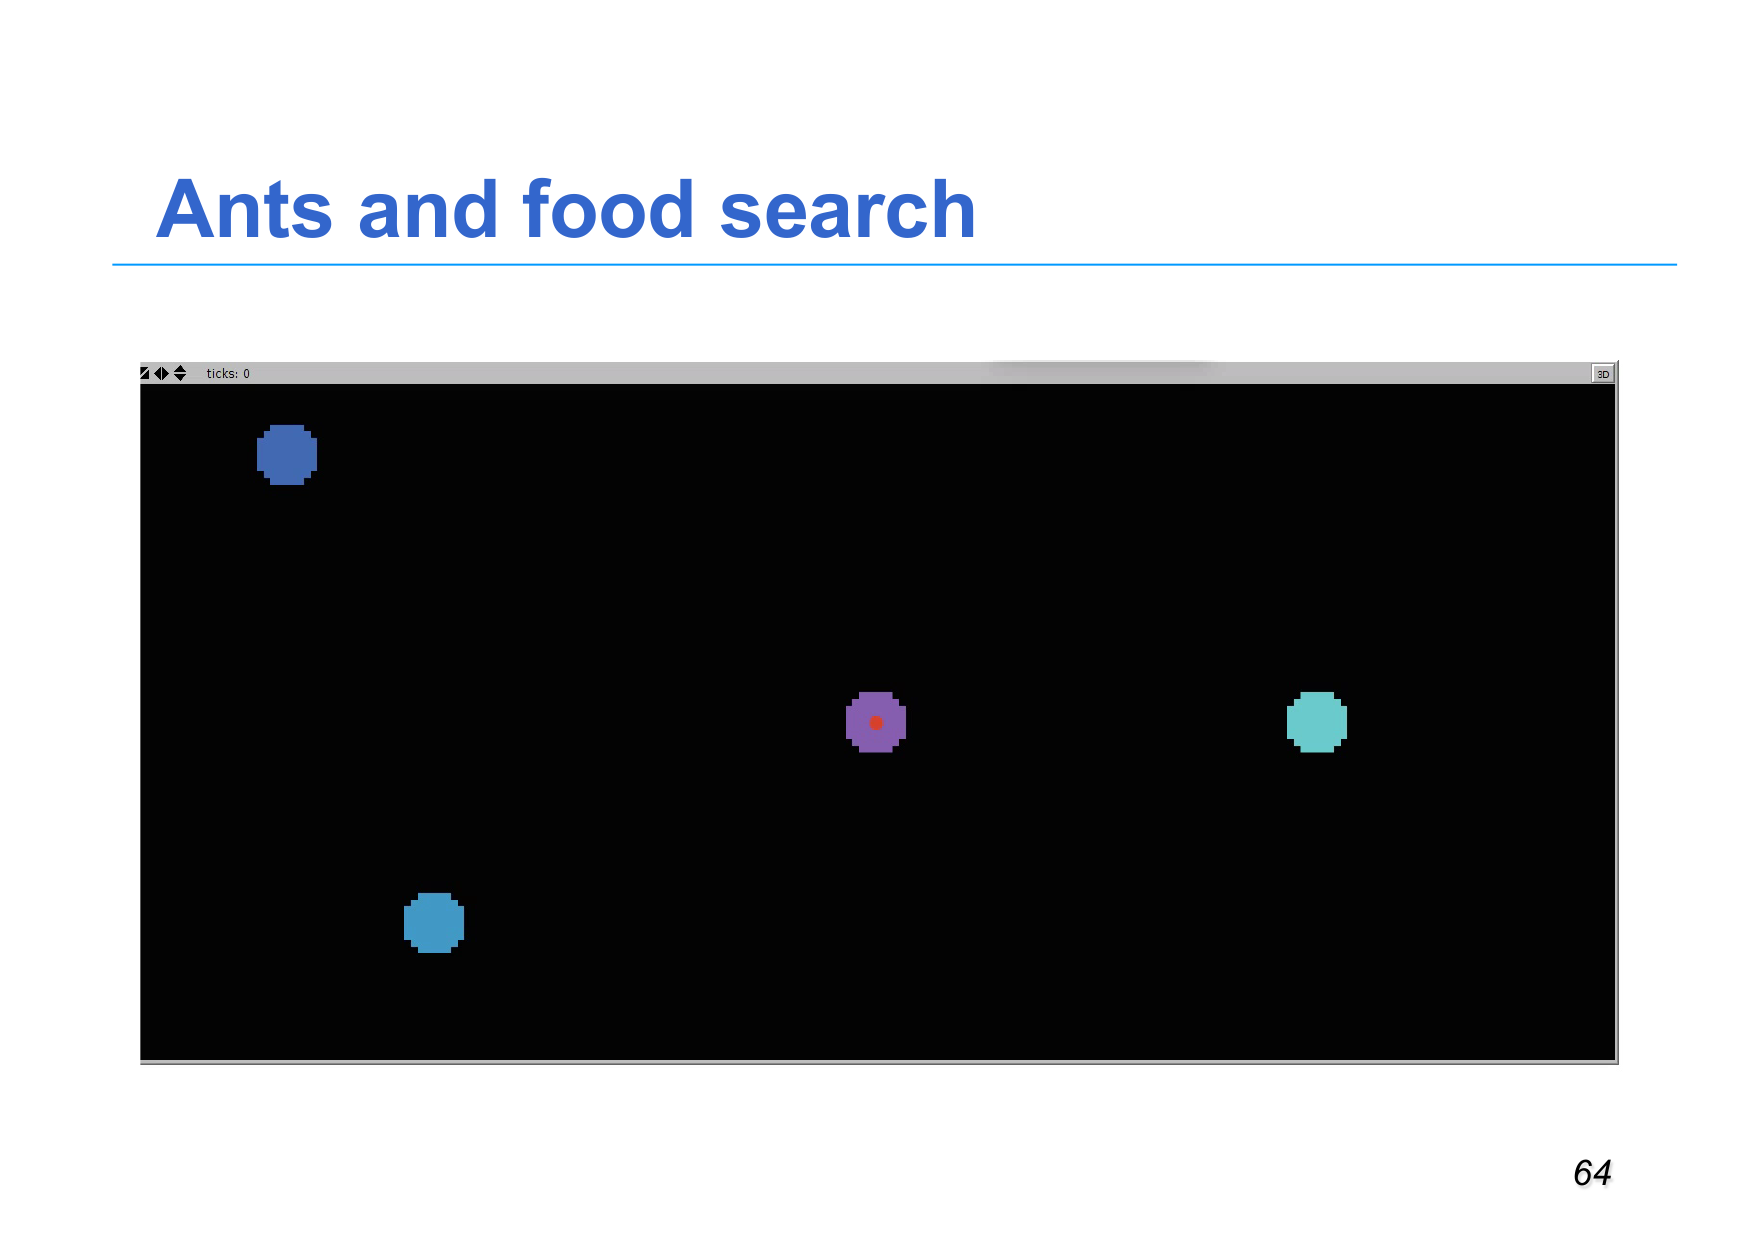
\includegraphics[width=0.75\textwidth]{img/formiche.png}
  \caption{Formiche e ricerca del cibo: il cammino più breve emerge dal deposito di
  feromone, senza alcun controllo centrale.}
\end{figure}

\subsection{Algoritmi genetici ed evolutivi}

\dfn{Algoritmo genetico}{
  Gli algoritmi genetici (e più in generale gli algoritmi evolutivi) sono ispirati
  all'\textbf{evoluzione naturale} e sono stati sviluppati negli anni '70 da
  \textbf{John Holland}.

  Si parte da una \textbf{popolazione iniziale casuale} di individui, che creano
  nuovi individui attraverso leggi specifiche (\textbf{cross-over} e
  \textbf{mutazione}).
}

\mprop{Operatori}{
  \begin{itemize}
    \item \textbf{Fitness}: garantisce che vengano mantenuti solo gli individui
      migliori;
    \item \textbf{Mutazione}: introduce nuovi elementi in modo casuale;
    \item \textbf{Cross-over}: combina buone soluzioni ``genitore''.
  \end{itemize}
  La fitness non è sempre facile da definire: in alcuni casi può essere
  \textbf{chiesta all'utente}.
}

\nt{
  Questi algoritmi sono utili quando è \textbf{difficile definire un modello} del
  problema.
}

\section{Reinforcement learning}

\dfn{Reinforcement learning}{
  Apprendimento di \textbf{policy}: come agire dato uno stato del sistema.
  Lo schema di controllo è:
  \[
    X_k \longrightarrow \text{Learner} \xrightarrow{\;Y_k\;}
    \text{Controlled System} \xrightarrow{\;Z_k\;}
  \]
  con un \textbf{Critic} che restituisce al learner il segnale di
  \textbf{rinforzo} $R$.

  \textbf{Rinforzo}: punizione o ricompensa.
}

\begin{figure}[H]
  \centering
  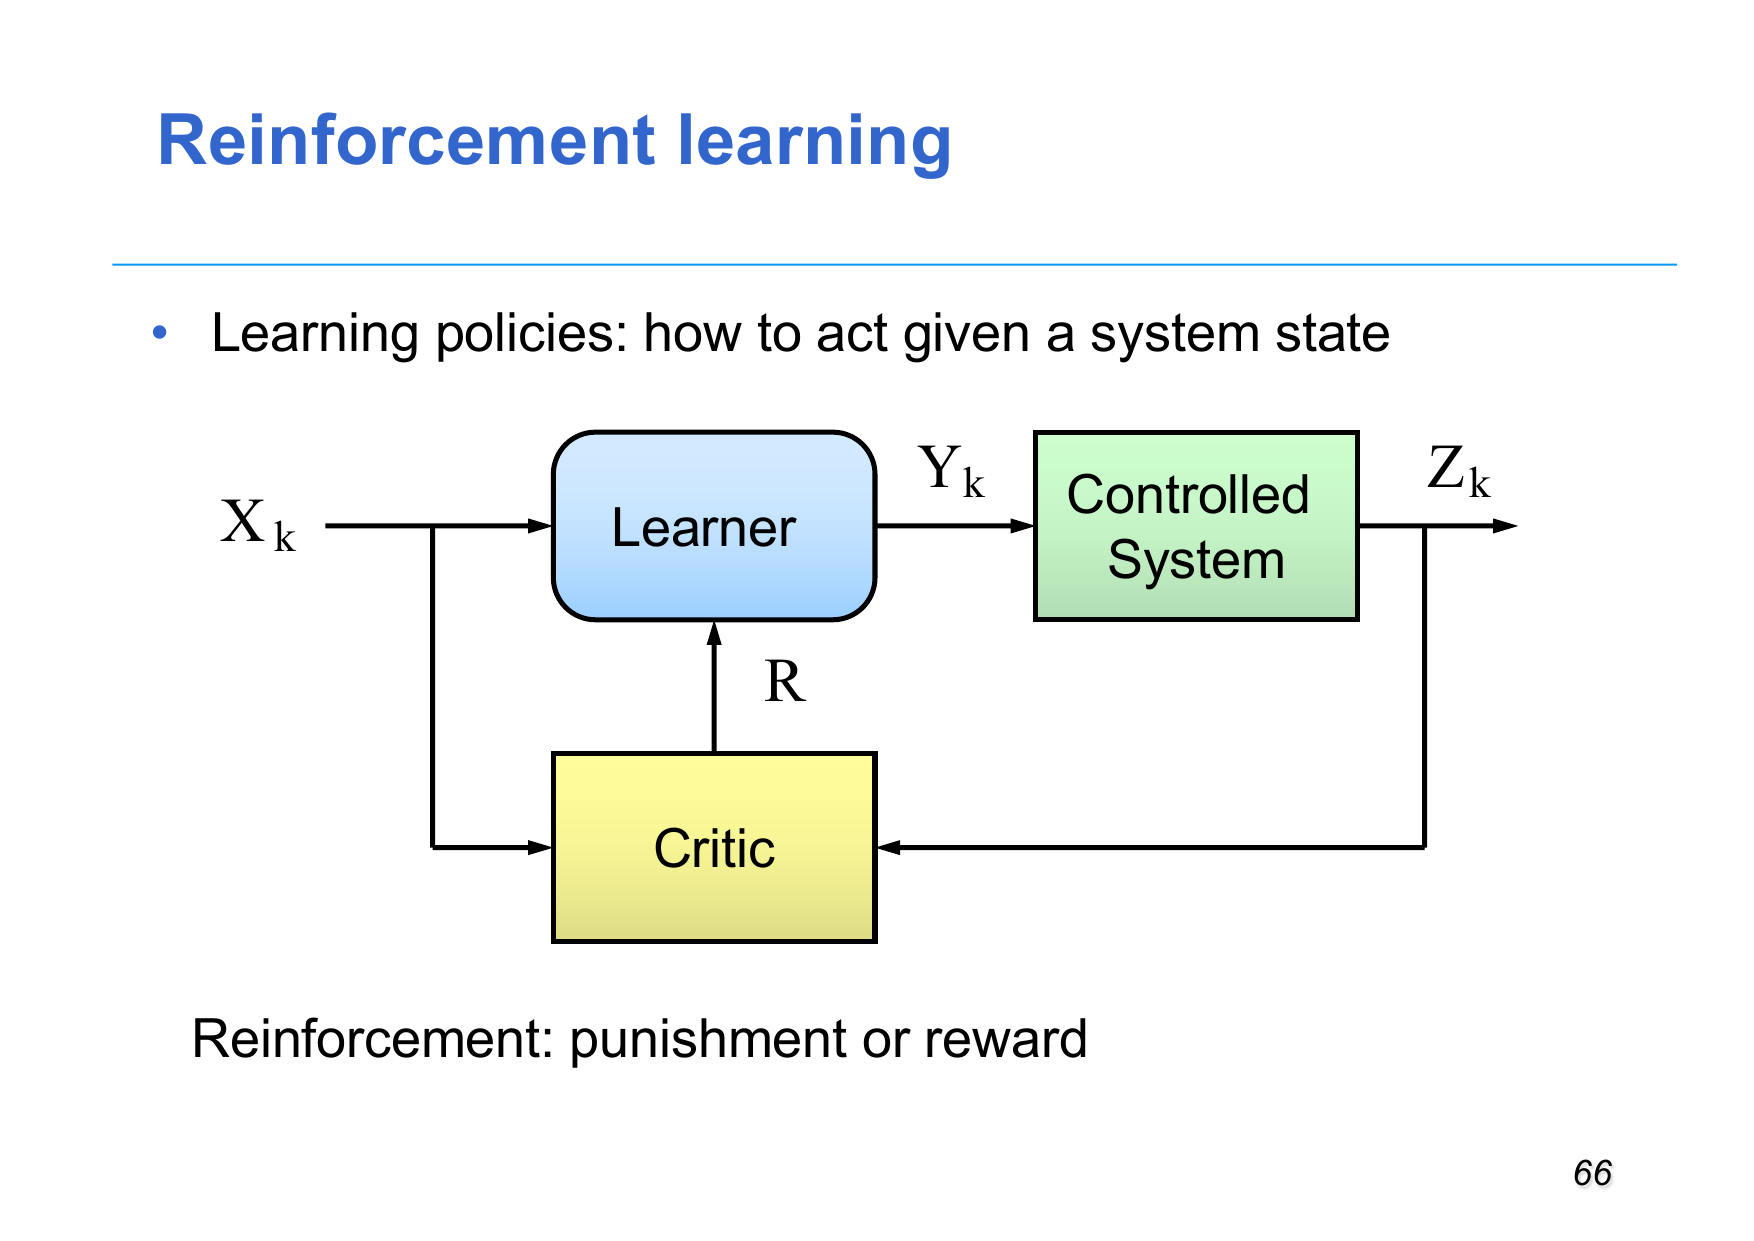
\includegraphics[width=0.75\textwidth]{img/rl-schema.png}
  \caption{Schema del reinforcement learning: learner, sistema controllato e critic.}
\end{figure}

\nt{
  Applicazione emblematica: \textbf{battere il campione del mondo} in un gioco
  (AlphaGo, Google Research). Il RL chiude il cerchio del corso, perché è
  contemporaneamente una tecnica di \textbf{machine learning} e una tecnica di
  \textbf{planning} (apprendimento di una policy).
}

\section{Riepilogo}

\nt{
  Mappa concettuale della lezione:
  \begin{itemize}
    \item \textbf{Che cos'è l'IA}: intelligenza $\to$ test di Turing $\to$
      weak/strong, general/narrow;
    \item \textbf{Due approcci}: simbolico (logica, regole, leggibile) vs
      connessionista (reti neurali, appreso da esempi, opaco);
    \item \textbf{Forme di ragionamento}: deduzione (corretta, non crea conoscenza),
      induzione (crea conoscenza, non corretta), abduzione (dalle cause agli
      effetti), analogia, vincoli;
    \item \textbf{Programmazione logica}: algoritmo = logica + controllo;
      Prolog, clausole di Horn, deduzione/induzione/abduzione nello stesso
      formalismo;
    \item \textbf{Machine learning}: supervisionato (classificazione, regressione),
      non supervisionato (clustering), con rinforzo;
    \item \textbf{Dal percettrone al deep learning}: separazione lineare $\to$
      regioni convesse $\to$ regioni arbitrarie $\to$ gerarchie di feature $\to$
      foundation model e agenti;
    \item \textbf{Planning}: stato iniziale, azioni con precondizioni ed effetti,
      goal; tecniche classiche e comportamenti emergenti.
  \end{itemize}
}

% \end{document}
